% --------------------------------------------------------------
% This is all preamble stuff that you don't have to worry about.
% Head down to where it says "Start here"
% --------------------------------------------------------------
 
%\documentclass[12pt]{article}
\documentclass[usletter,12pt]{article}
\usepackage[utf8]{inputenc}
\usepackage{setspace}
\usepackage{graphicx}
\usepackage{subcaption}
%\usepackage[T1,T2A]{fontenc}
\usepackage{hyperref}
\usepackage[margin=1in]{geometry} 
\usepackage{amsmath,amsthm,amssymb}
\usepackage{listings} 
\renewcommand*{\ttdefault}{qcr}
\usepackage{tgcursor}
\lstset{basicstyle=\footnotesize\ttfamily,breaklines=true}
\usepackage{lipsum}
\lstset{breaklines=true}
\usepackage{courier}

\newcommand{\N}{\mathbb{N}}
\newcommand{\Z}{\mathbb{Z}}
 
\newenvironment{theorem}[2][Theorem]{\begin{trivlist}
\item[\hskip \labelsep {\bfseries #1}\hskip \labelsep {\bfseries #2.}]}{\end{trivlist}}
\newenvironment{lemma}[2][Lemma]{\begin{trivlist}
\item[\hskip \labelsep {\bfseries #1}\hskip \labelsep {\bfseries #2.}]}{\end{trivlist}}
\newenvironment{exercise}[2][Exercise]{\begin{trivlist}
\item[\hskip \labelsep {\bfseries #1}\hskip \labelsep {\bfseries #2.}]}{\end{trivlist}}
\newenvironment{reflection}[2][Reflection]{\begin{trivlist}
\item[\hskip \labelsep {\bfseries #1}\hskip \labelsep {\bfseries #2.}]}{\end{trivlist}}
\newenvironment{proposition}[2][Proposition]{\begin{trivlist}
\item[\hskip \labelsep {\bfseries #1}\hskip \labelsep {\bfseries #2.}]}{\end{trivlist}}
\newenvironment{corollary}[2][Corollary]{\begin{trivlist}
\item[\hskip \labelsep {\bfseries #1}\hskip \labelsep {\bfseries #2.}]}{\end{trivlist}}
 
\begin{document}
 
% --------------------------------------------------------------
%                         Start here
% --------------------------------------------------------------
 
%\renewcommand{\qedsymbol}{\filledbox}
 
\title{Project 1: Hot Wire(less)}%replace X with the appropriate number
\author{Yuding Ai  \\Penn ID: 31295008\\ %replace with your name
CIS 553 - Networked Systems} %if necessary, replace with your course title
\maketitle
\section{Phase 1: Take 5}
In Phase 1, we found 5 WAPs (Wifi access point) and recorded the BSSIDs and origin locations (lat./long.) However, I later realized that the origin locations I found last time are not accurate enough, so this time I choose the \textbf{location with strongest signal to be as the origin of the WAPs} and attach them again in this final report as below. (the BSSIDs are the same as in my Phase 1 email though.) \\\textbf{5 WAPs for Phase 1:}
\begin{enumerate}
\item BSSID1 84:d4:7e:dc:2a:40, Latitude: 39.95233362, Longitude: -75.19346528
\item BSSID2 94:b4:0f:53:07:00, Latitude: 39.95322759, Longitude: -75.19217689 
\item BSSID3 ac:86:74:57:d6:82, Latitude: 39.95303359, Longitude: -75.19318620
\item BSSID4 e2:55:7d:46:ba:70, Latitude: 39.95348435, Longitude: -75.19542690
\item BSSID5 e8:40:40:80:52:e8, Latitude: 39.95339425, Longitude: -75.19608680
\label{enu}
\end{enumerate}
\section{Phase 2: Tower of Power}
In Phase 2, we collected power levels (in dBm) for the 5 WAPs found in Phase 1 with more than 20 locations each. Furthermore, besides the required BSSID, Lat, Long and power(in dBm), I have also included the distance in meters (\textbf{Dis})\footnote{distance is calculated using the so called Harversine formula, see detailed calculation in python source code and see reference:http://www.movable-type.co.uk/scripts/latlong.html} from each location to its WAP origin and the `ideal' signal strength in dBm (\textbf{Rpower}) in Free space, calculated through the idea of $Power \propto \frac{1}{r^2}$, where r is the distance from the location to its WAP origin. To calculate this so-called Rpower, we first convert the power of the origin from dBm into mW and compute the Rpower for the target location in mW, and then converted it back to dBm as to make comparison with the observed data(the actual signal I measured using my Android phone with the wigle app). \autoref{unit} describes how dBm converted to mW, and vice versa where x is in unit of dBm and P is in unit of mW.
\begin{eqnarray}
x = 10\log_{10} \frac{P}{1 mW} \nonumber \\
P = 1mW \times 10^{\frac{x}{10}}
\label{unit}
\end{eqnarray}
So for example: if the origin has a Power of -41 dBm, when converted into mW, it should be 0.000079432823472 mW. An location that is 7.04 meters away from the origin, should have $Rpower =  0.000079432823472 \times \frac{1}{7.04^2} = 1.6027\times10^{-6}\ mW = -57.95\ dBm$
\lstinputlisting[language=Python,  breaklines=true,caption=WAP1\_Library]{library.txt}
\lstinputlisting[language=Python,  breaklines=true,caption=WAP2\_Starbucks]{starbucks.txt}
\lstinputlisting[language=Python,  breaklines=true,caption=WAP3\_United\_by\_blue]{unitedblue.txt}
\lstinputlisting[language=Python,  breaklines=true,caption=WAP4\_Bluemercury]{bluemercury.txt}
\lstinputlisting[language=Python,  breaklines=true,caption=WAP5\_PenneBar]{penne.txt}
Using the above data, we could simply plot Power VS Distance as to compare the measured Wifi signal strength with the ideal signal strength. Such result is depicted in
\autoref{fig:plot1&2}, \autoref{fig:plot3&4} and \autoref{fig:plot5}.\\\\
Next we compare the attenuation at each point to what the $1/r^2$ model would predict. As is shown in the Power VS Distance plots for Library, and Penne-bar, almost always, the measured Wifi signal strength is a bit weaker than the Ideal signal strength (indicates the actual signal attenuation is greater then $1/r^2$ model), such that the average bulk propagation loss is a little greater than what $1/r^2$ predicts and this result is expected due to the fact that the real world is not a ``free space", so that signals will be reflected and bounced back or block by obstacles, thus that the actual signal is a bit weaker then the ideal case predicted by $Power \propto \frac{1}{r^2}$. Nevertheless, for some other plots, such like the starbucks one, we see that for about half of the times, the measured signal are actually greater than ideal case (and they are not supposed to be) and this could be explained by an inaccurate measurement of origin location and origin signal strength since the Wifi router of Starbucks is actually located inside the building, but once we get into a building, we lost the GPS signal so it cause the inaccuracy. And so does all my other WAPs except for the one from Library. My target Library router is located near the glass wall of the underground floor, which is very close to outside so that I could get a relatively more accurate location and signal strength from outside.
\\\\
\begin{figure}[!h]
	\begin{subfigure}{0.5\textwidth}
		\centering
		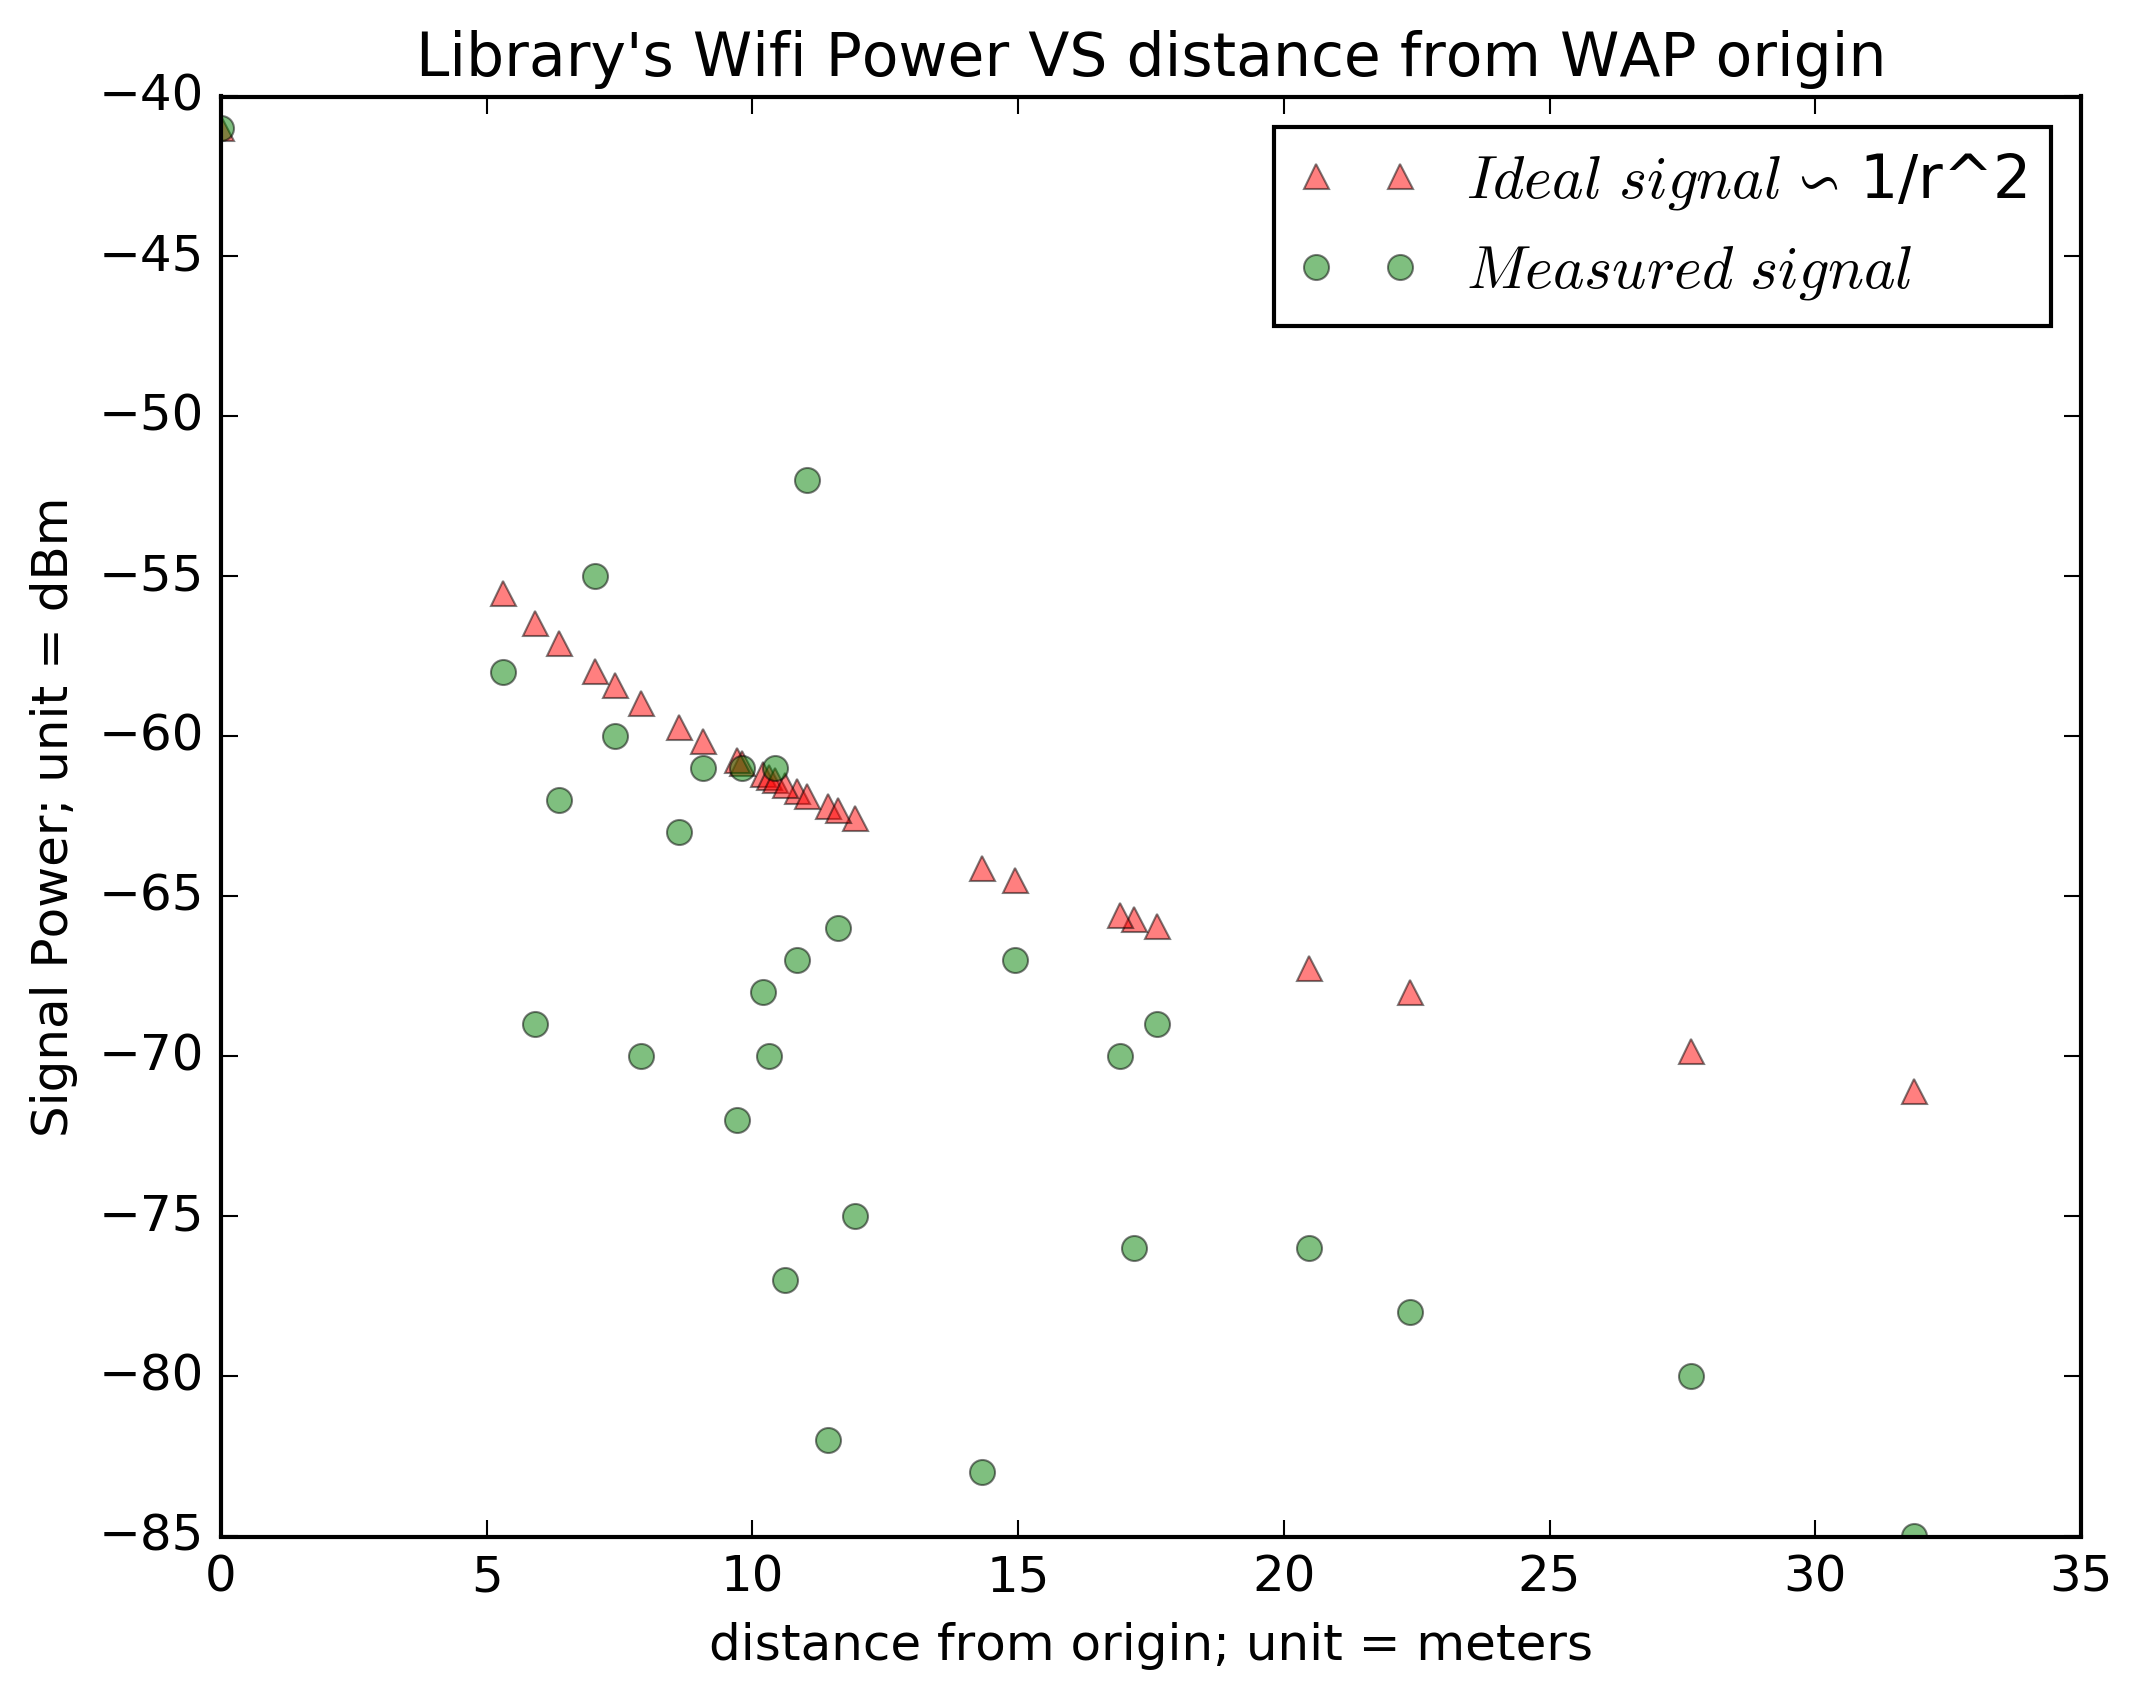
\includegraphics[width=1\linewidth, height=7cm]{Librarypower.png} 
		\caption{Library Power vs Distance}
	\end{subfigure}
	\begin{subfigure}{0.5\textwidth}
	    \centering
		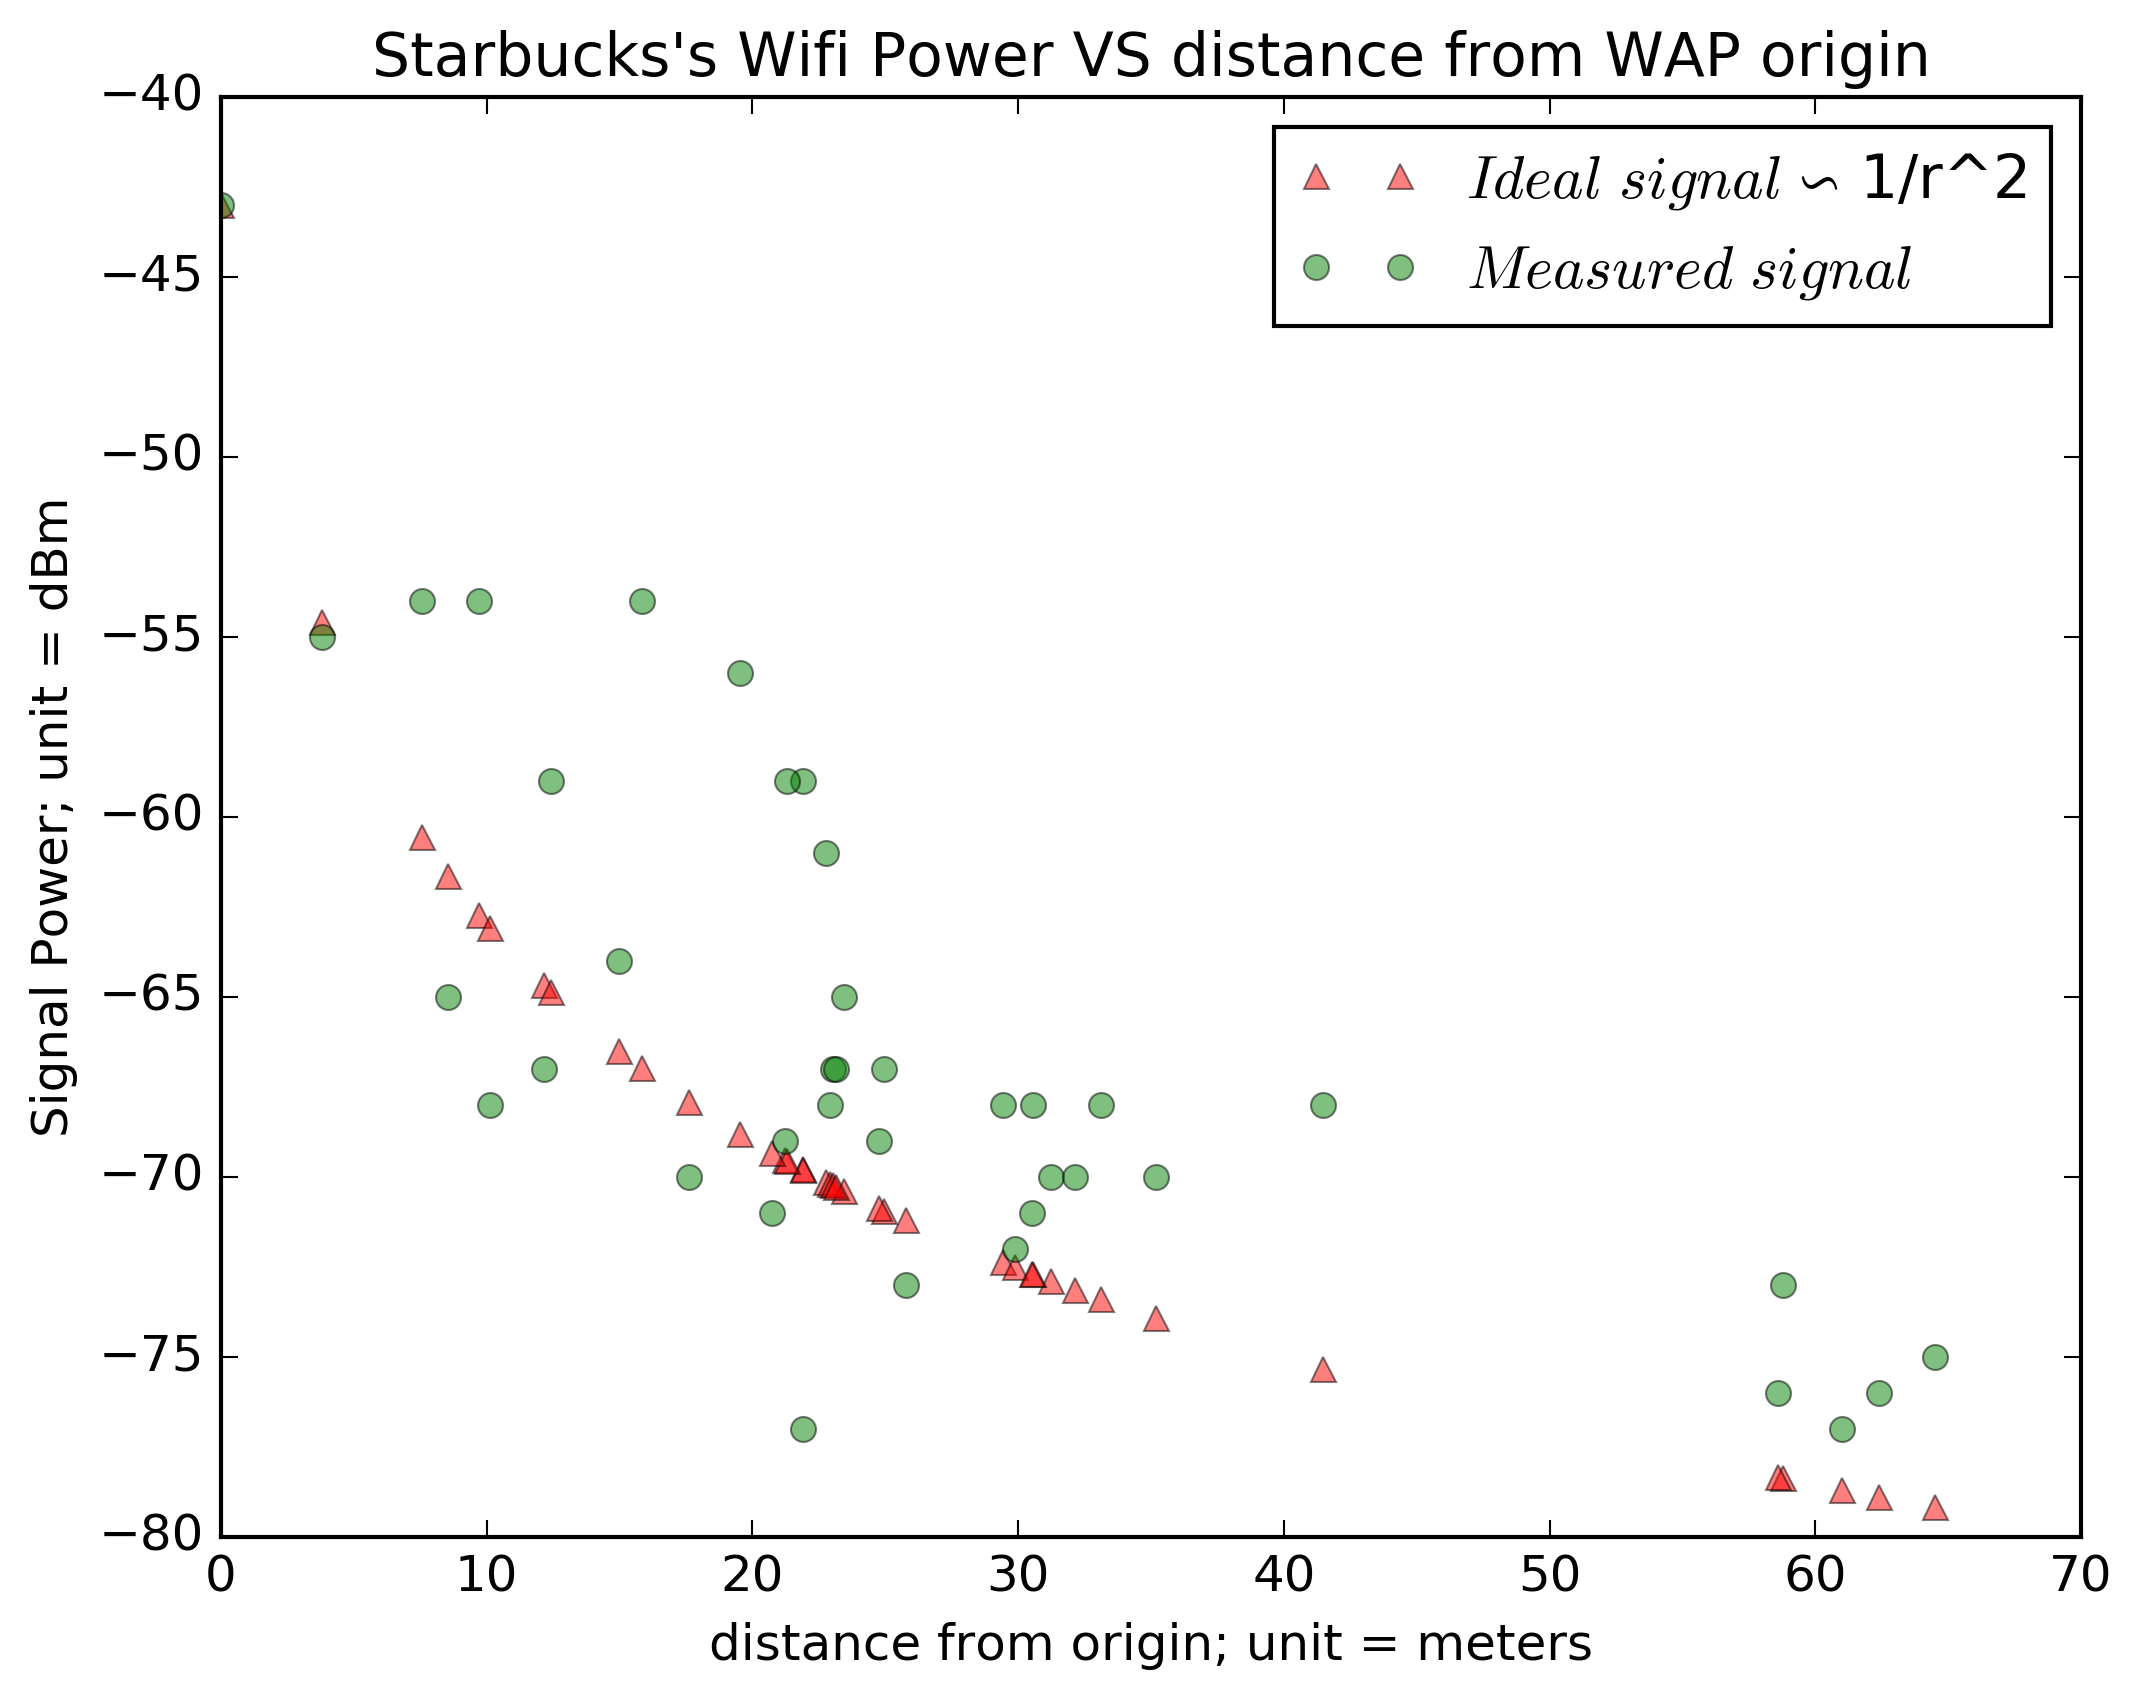
\includegraphics[width=1\linewidth, height=7cm]{Starbuckspower.png}
		\caption{Starbucks Power vs Distance}
	\end{subfigure}
	\caption{Library and Starbucks}
	\label{fig:plot1&2}
\end{figure}
\begin{figure}[!h]
	\begin{subfigure}{0.5\textwidth}
		\centering
		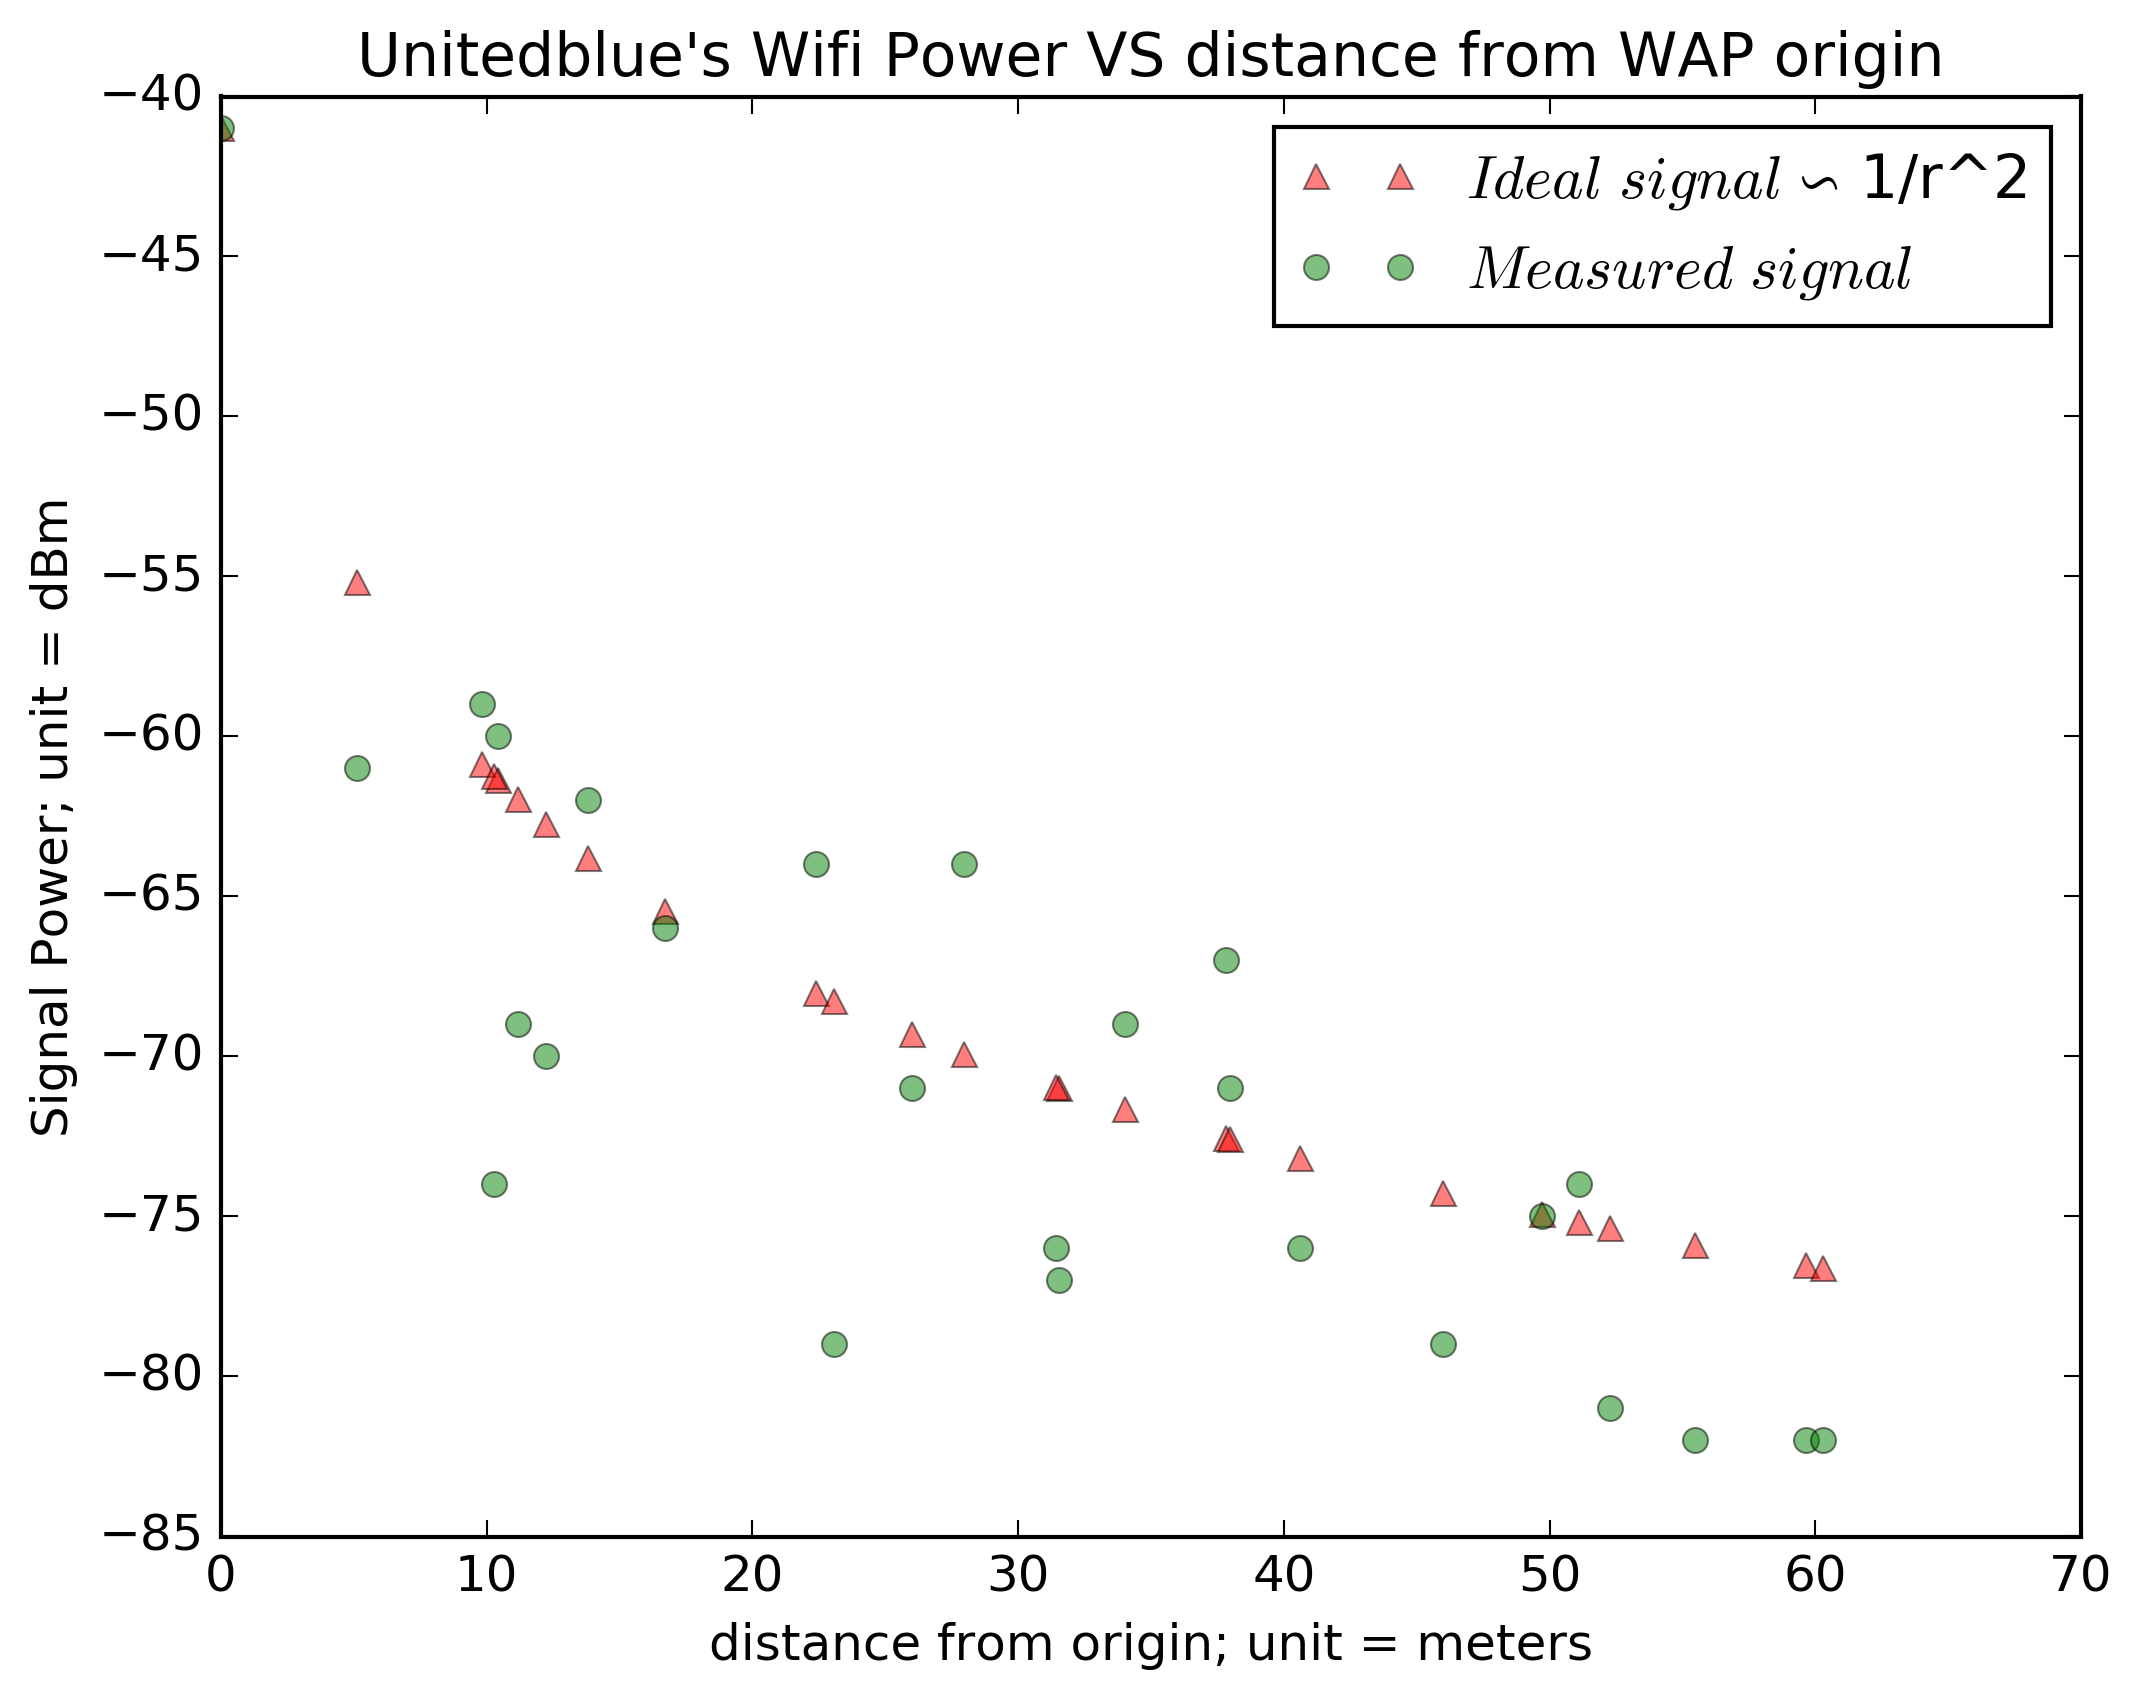
\includegraphics[width=1\linewidth, height=7cm]{Unitedbluepower.png} 
		\caption{United by Blue Power vs Distance}
	\end{subfigure}
	\begin{subfigure}{0.5\textwidth}
	    \centering
		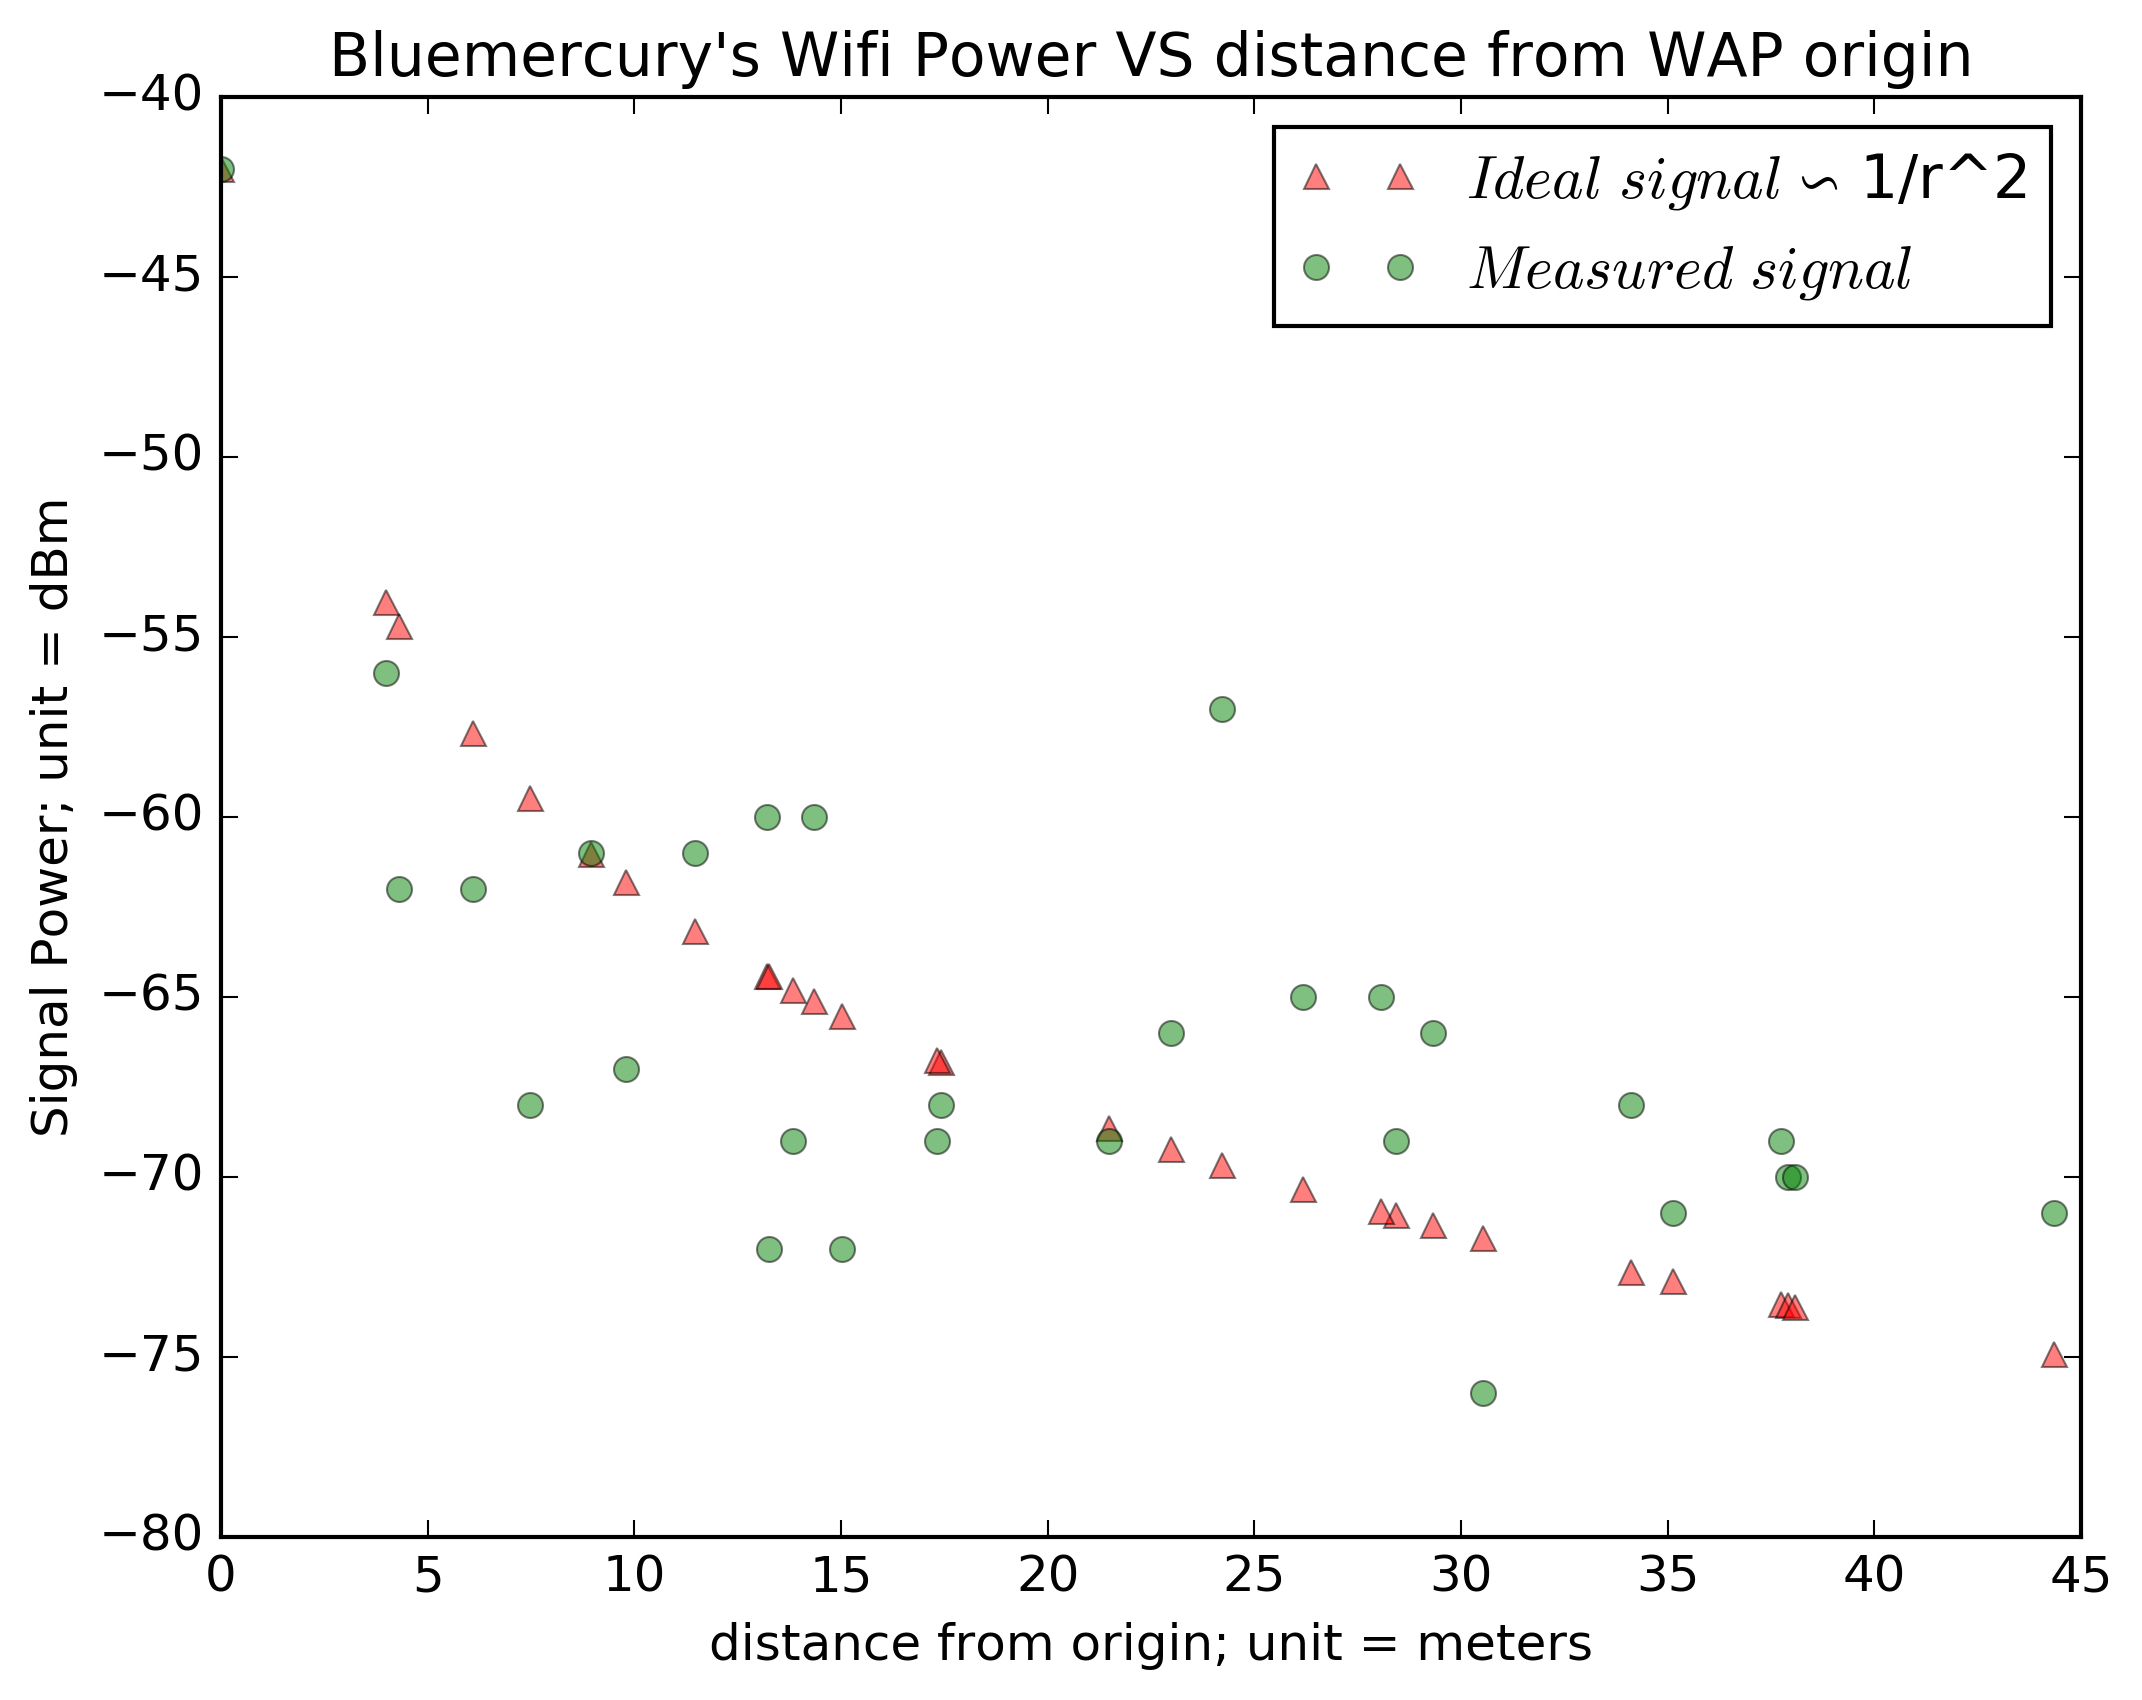
\includegraphics[width=1\linewidth, height=7cm]{Bluemercurypower.png}
		\caption{Bluemercury Power vs Distance}
	\end{subfigure}
	\caption{United by Blue and Bluemercury Power vs Distance}
	\label{fig:plot3&4}
\end{figure}
\begin{figure}[!h]
	\centering
	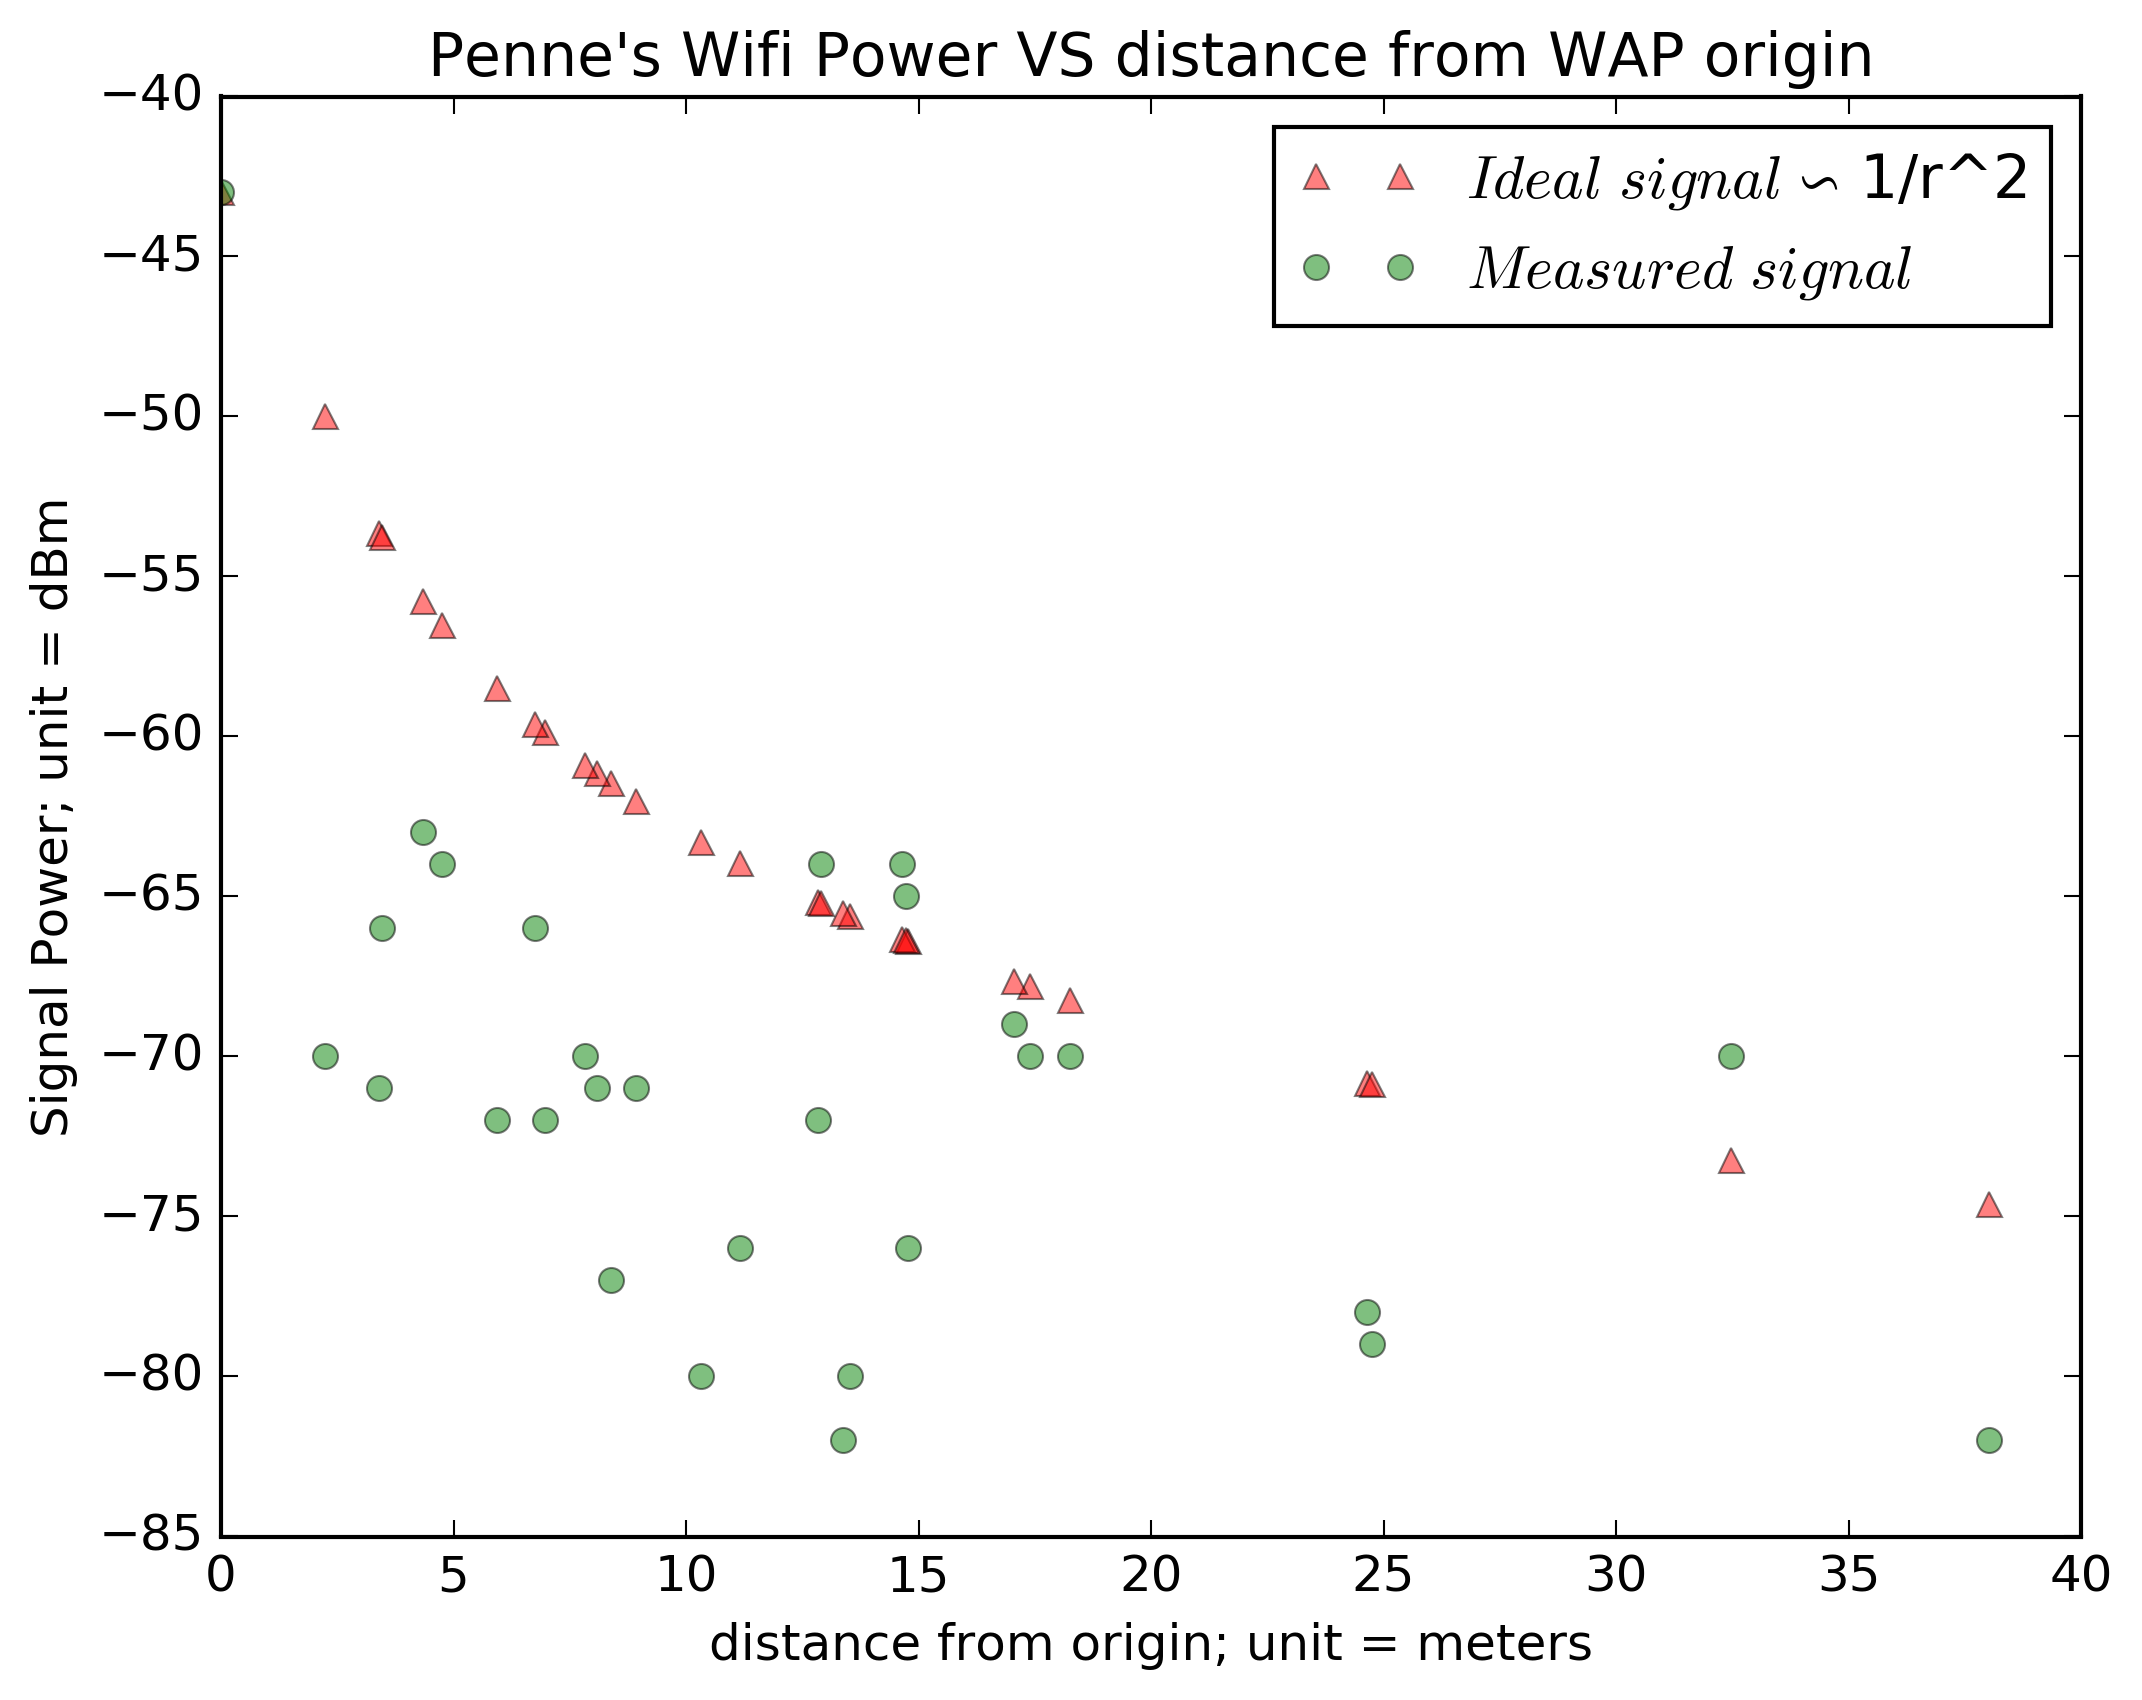
\includegraphics[width=1\linewidth]{Pennepower.png}
	\caption{Penne-bar Power vs Distance}
\label{fig:plot5}
\end{figure}

\clearpage
\subsection{Calculate the Average bulk propagation loss}
I add this section on Feb 20 as to include the calculation for average bulk propagation. All calculation is based on Piazza post @64 and assume the noise power to be $P_{noise} = -100dBm = 10^{-10} mW$.\\\\
To calculate the Signal power to noise ratio in dB, we use \autoref{nratio}.\\
\begin{equation}
SNR_{dB} = 10\log_{10}(P_{r}/P_{noise})
\label{nratio}
\end{equation}
such that we could obtain the SNR by plugging the signal power (in mW) for each WAP into $P_{r}$. (Applies to both the measured signal power and the theoretical signal power predicted by $1/r^2$, so my Rpower). Then we assume\\
\begin{equation}
SNR = \frac{k}{r^2}
\end{equation} 
thus that the average bulk propagation loss $k_{ave}$ could then be obtained by taking the average of all k values. (k in unit of $dB*m^2$.).\\Finally, we attached the calculated Average bulk propagation loss along with the propagation loss (k) for each location as below:\\\\
\lstinputlisting[language=Python,  breaklines=true,caption=Propagation\_Loss\_Library]{libaveloss.txt}
\lstinputlisting[language=Python,  breaklines=true,caption=Propagation\_Loss\_Starbucks]{staraveloss.txt}
\lstinputlisting[language=Python,  breaklines=true,caption=Propagation\_Loss\_Unitedbyblue]{unitedaveloss.txt}
\lstinputlisting[language=Python,  breaklines=true,caption=Propagation\_Loss\_Blue\_mercury]{blueaveloss.txt}
\lstinputlisting[language=Python,  breaklines=true,caption=Propagation\_Loss\_Penne\_Bar]{penneaveloss.txt}
As is shown in those propagation loss (k) data, Once again, For Library, United by blue and Penne-bar, the result indicates that the average bulk propagation loss is a little greater than what $1/r^2$ predicts and this result is expected due to the fact that the real world is not a ``free space", so that signals will be reflected and bounced back or block by obstacles, thus that the actual signal is a bit weaker then the ideal case predicted by $Power \propto \frac{1}{r^2}$. (same conclusion as before). And for Starbucks and Blue mercury, due to the reason of inaccurate measurement of WAP origin location and its signal power, the propagation loss seems to be a bit smaller then what $1/r^2$ predicts.
\section{Phase 3: Peak Performance}
First of all, utilizing the Latitude and Longitude data we recorded in phase 2, we draw those locations directly onto google map\footnote{Using a little python package called gmplot, see reference https://github.com/vgm64/gmplot} as a scatter plot to show where those measured locations are. (I am actually a little bit surprised by the great accuracy of my GPS) Such plot is depicted in \autoref{fig:plot6}, where the dark purple dots are for Van Pelt Library, Green for Starbucks, Red for a cafe called `united by blue', Blue for a beauty retailer named Bluemurcury and Magenta for a restaurant named `Penne-bar'.
\begin{figure}[!h]
	\centering
	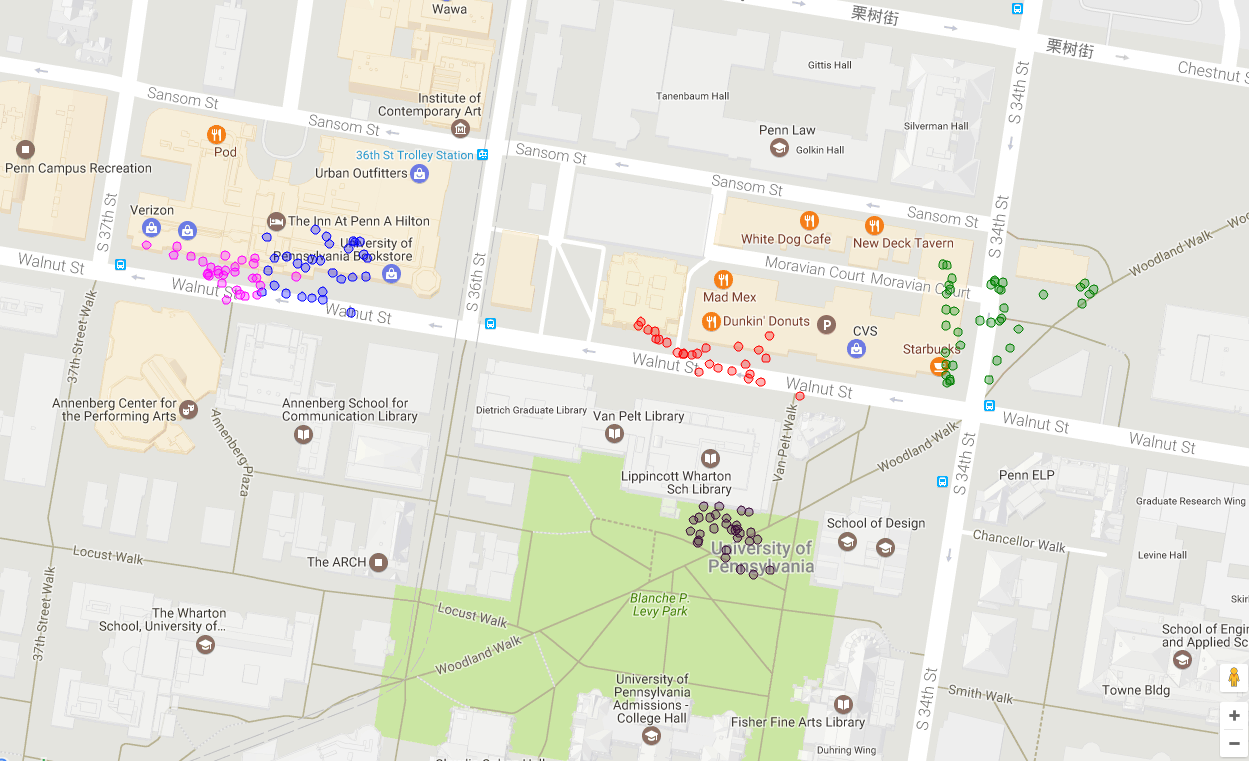
\includegraphics[width=1\linewidth]{Googlescatter.png}
	\caption{WAP Location Scatters on Google map}
\label{fig:plot6}
\end{figure}
\\
Then we plot the data from phase 2 as a heat map for each access points where the WAP origin location is marked as a green diamond symbol and a more reddish color indicates a stronger Wifi signal while a more bluish color stands for a weaker Wifi signal.(Notice that the `pattern shape' of each plots matched with the scatter plots on google map) Such plots are draw in \autoref{fig:plot7&8} for Library and Starbucks, \autoref{fig:plot9&10} for united by blue and bluemercury and \autoref{fig:plot11} for penne-bar.\\\\
As is shown in those plots, we see that spots that are close to the origin remain strong enough for online surfing (more than -60 dBm) while the spots that are further away from the origin became weaker(more bluish) and weaker.(agree with the theory) Therefore, such behavior of the Wifi signal is as expected.
\begin{figure}[!h]
	\begin{subfigure}{0.5\textwidth}
		\centering
		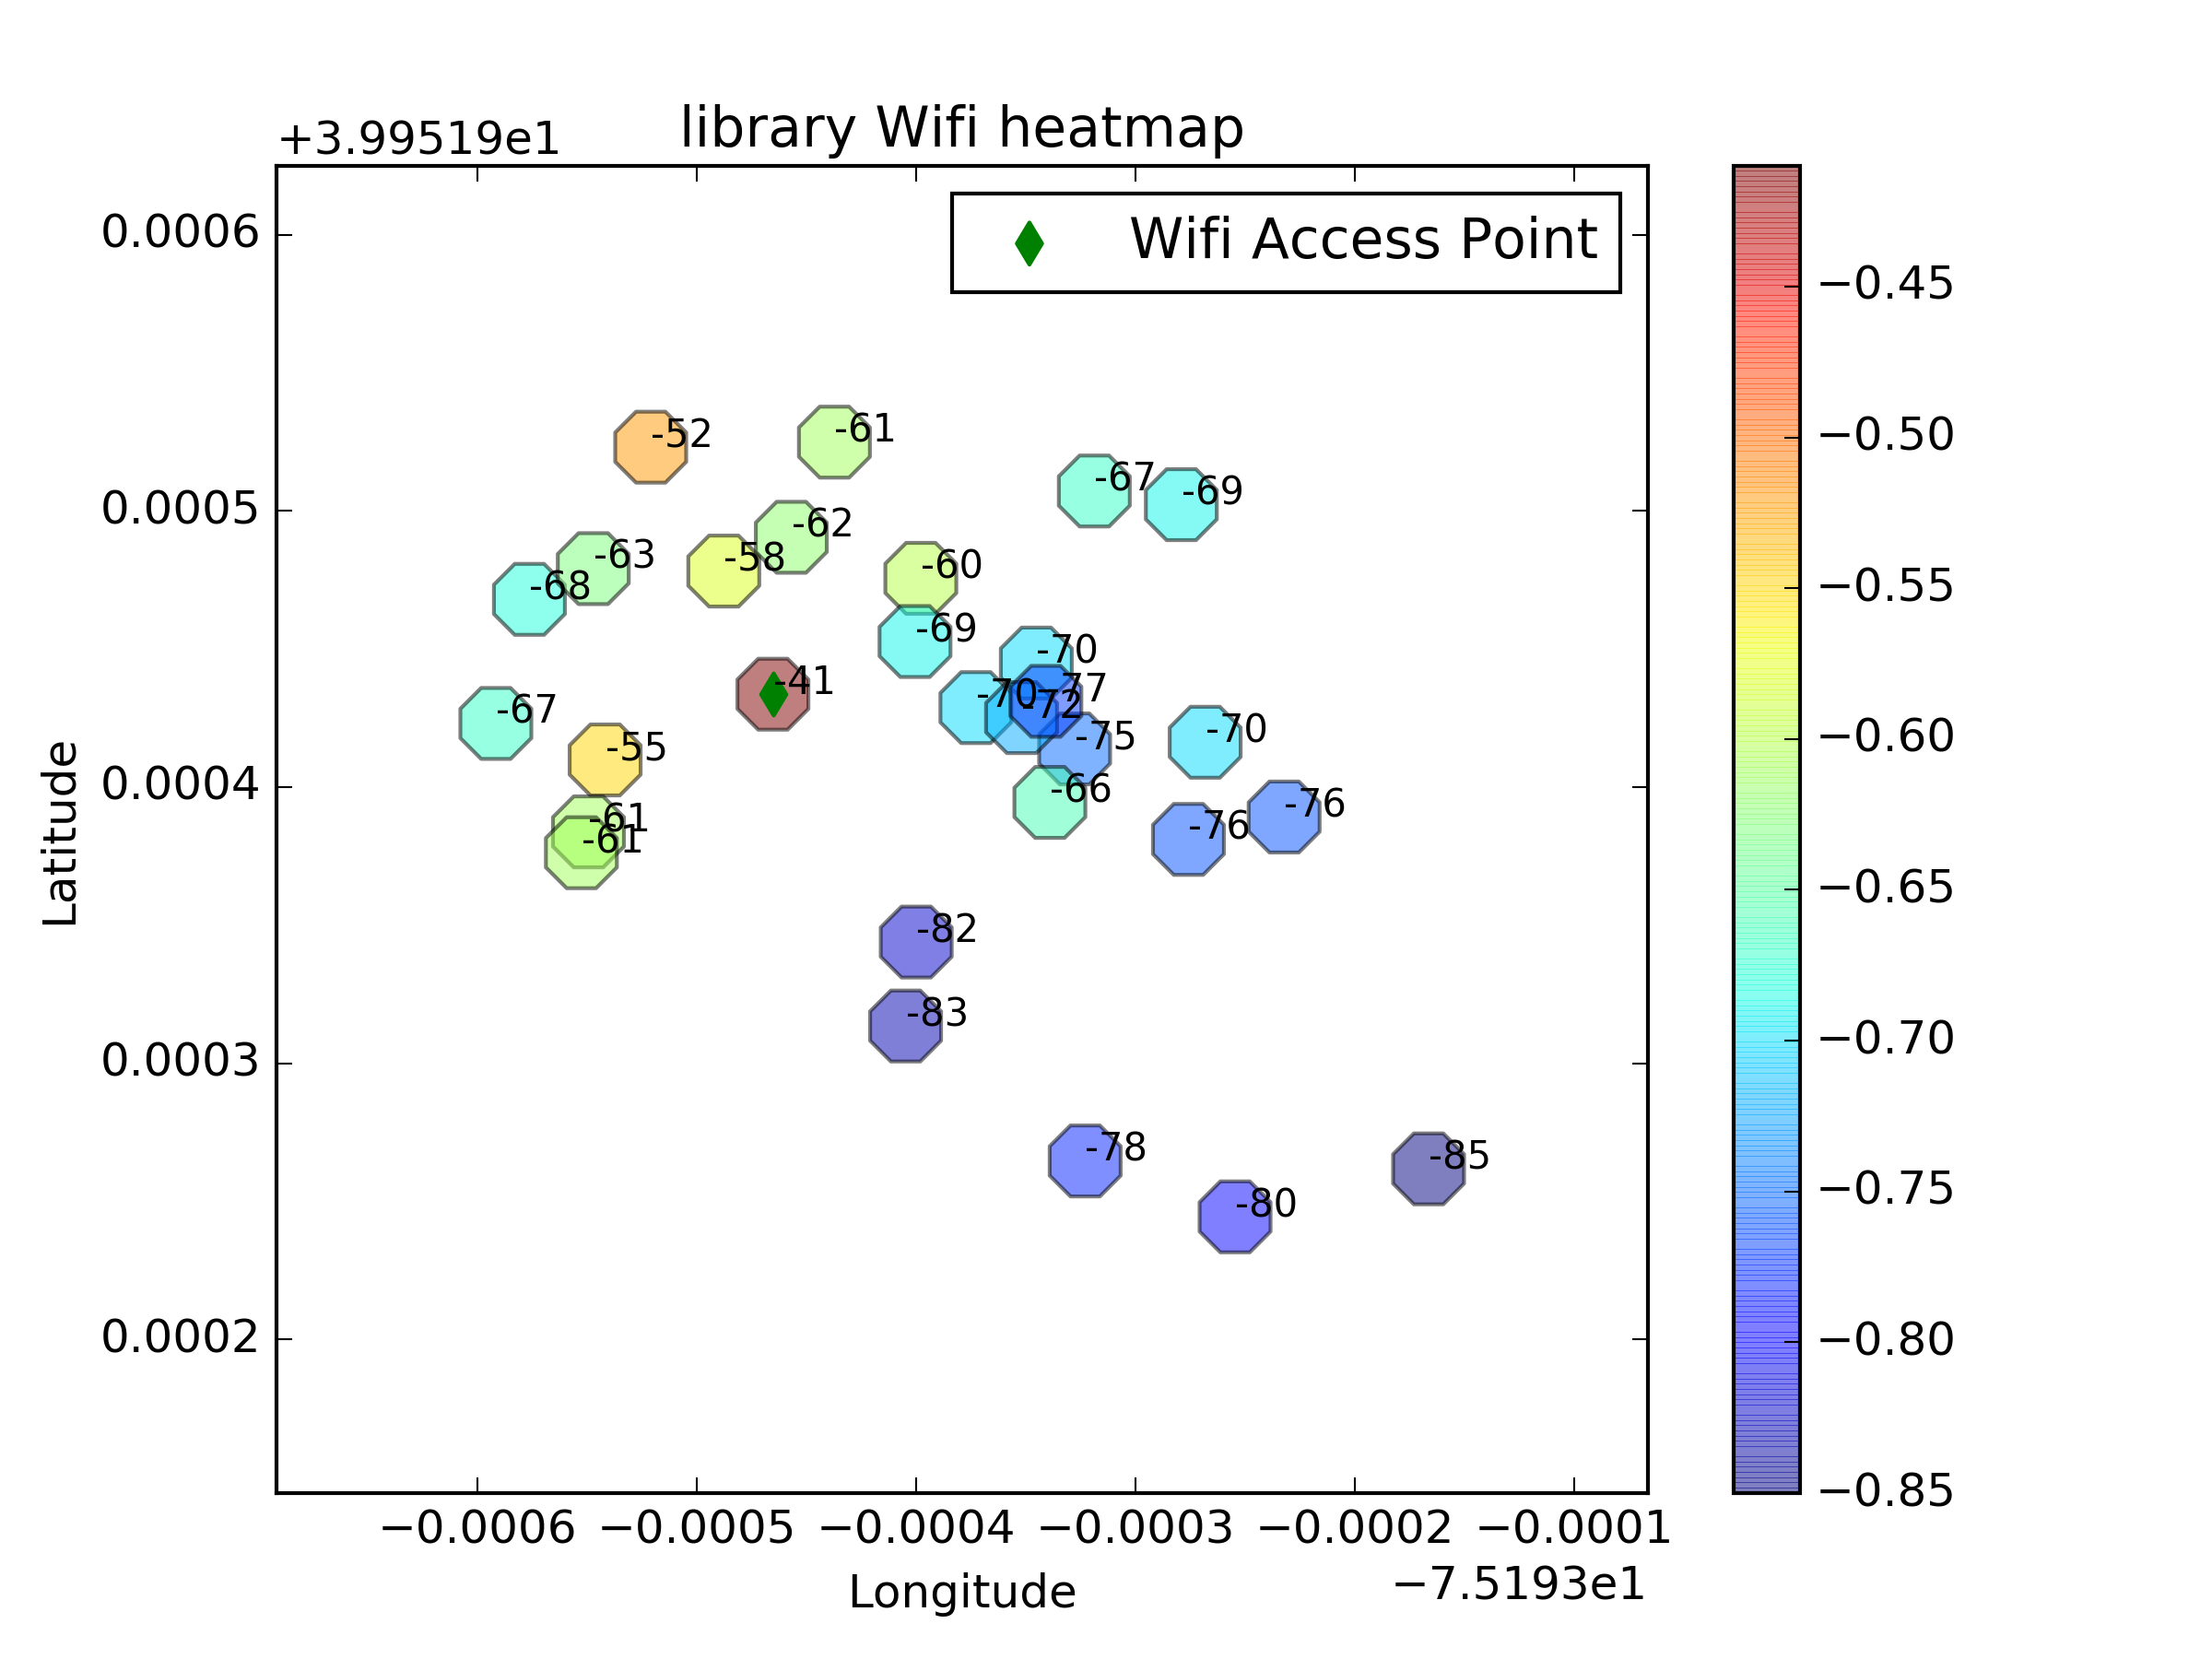
\includegraphics[width=1\linewidth, height=6cm]{library.png} 
		\caption{Library Heat map}
	\end{subfigure}
	\begin{subfigure}{0.5\textwidth}
	    \centering
		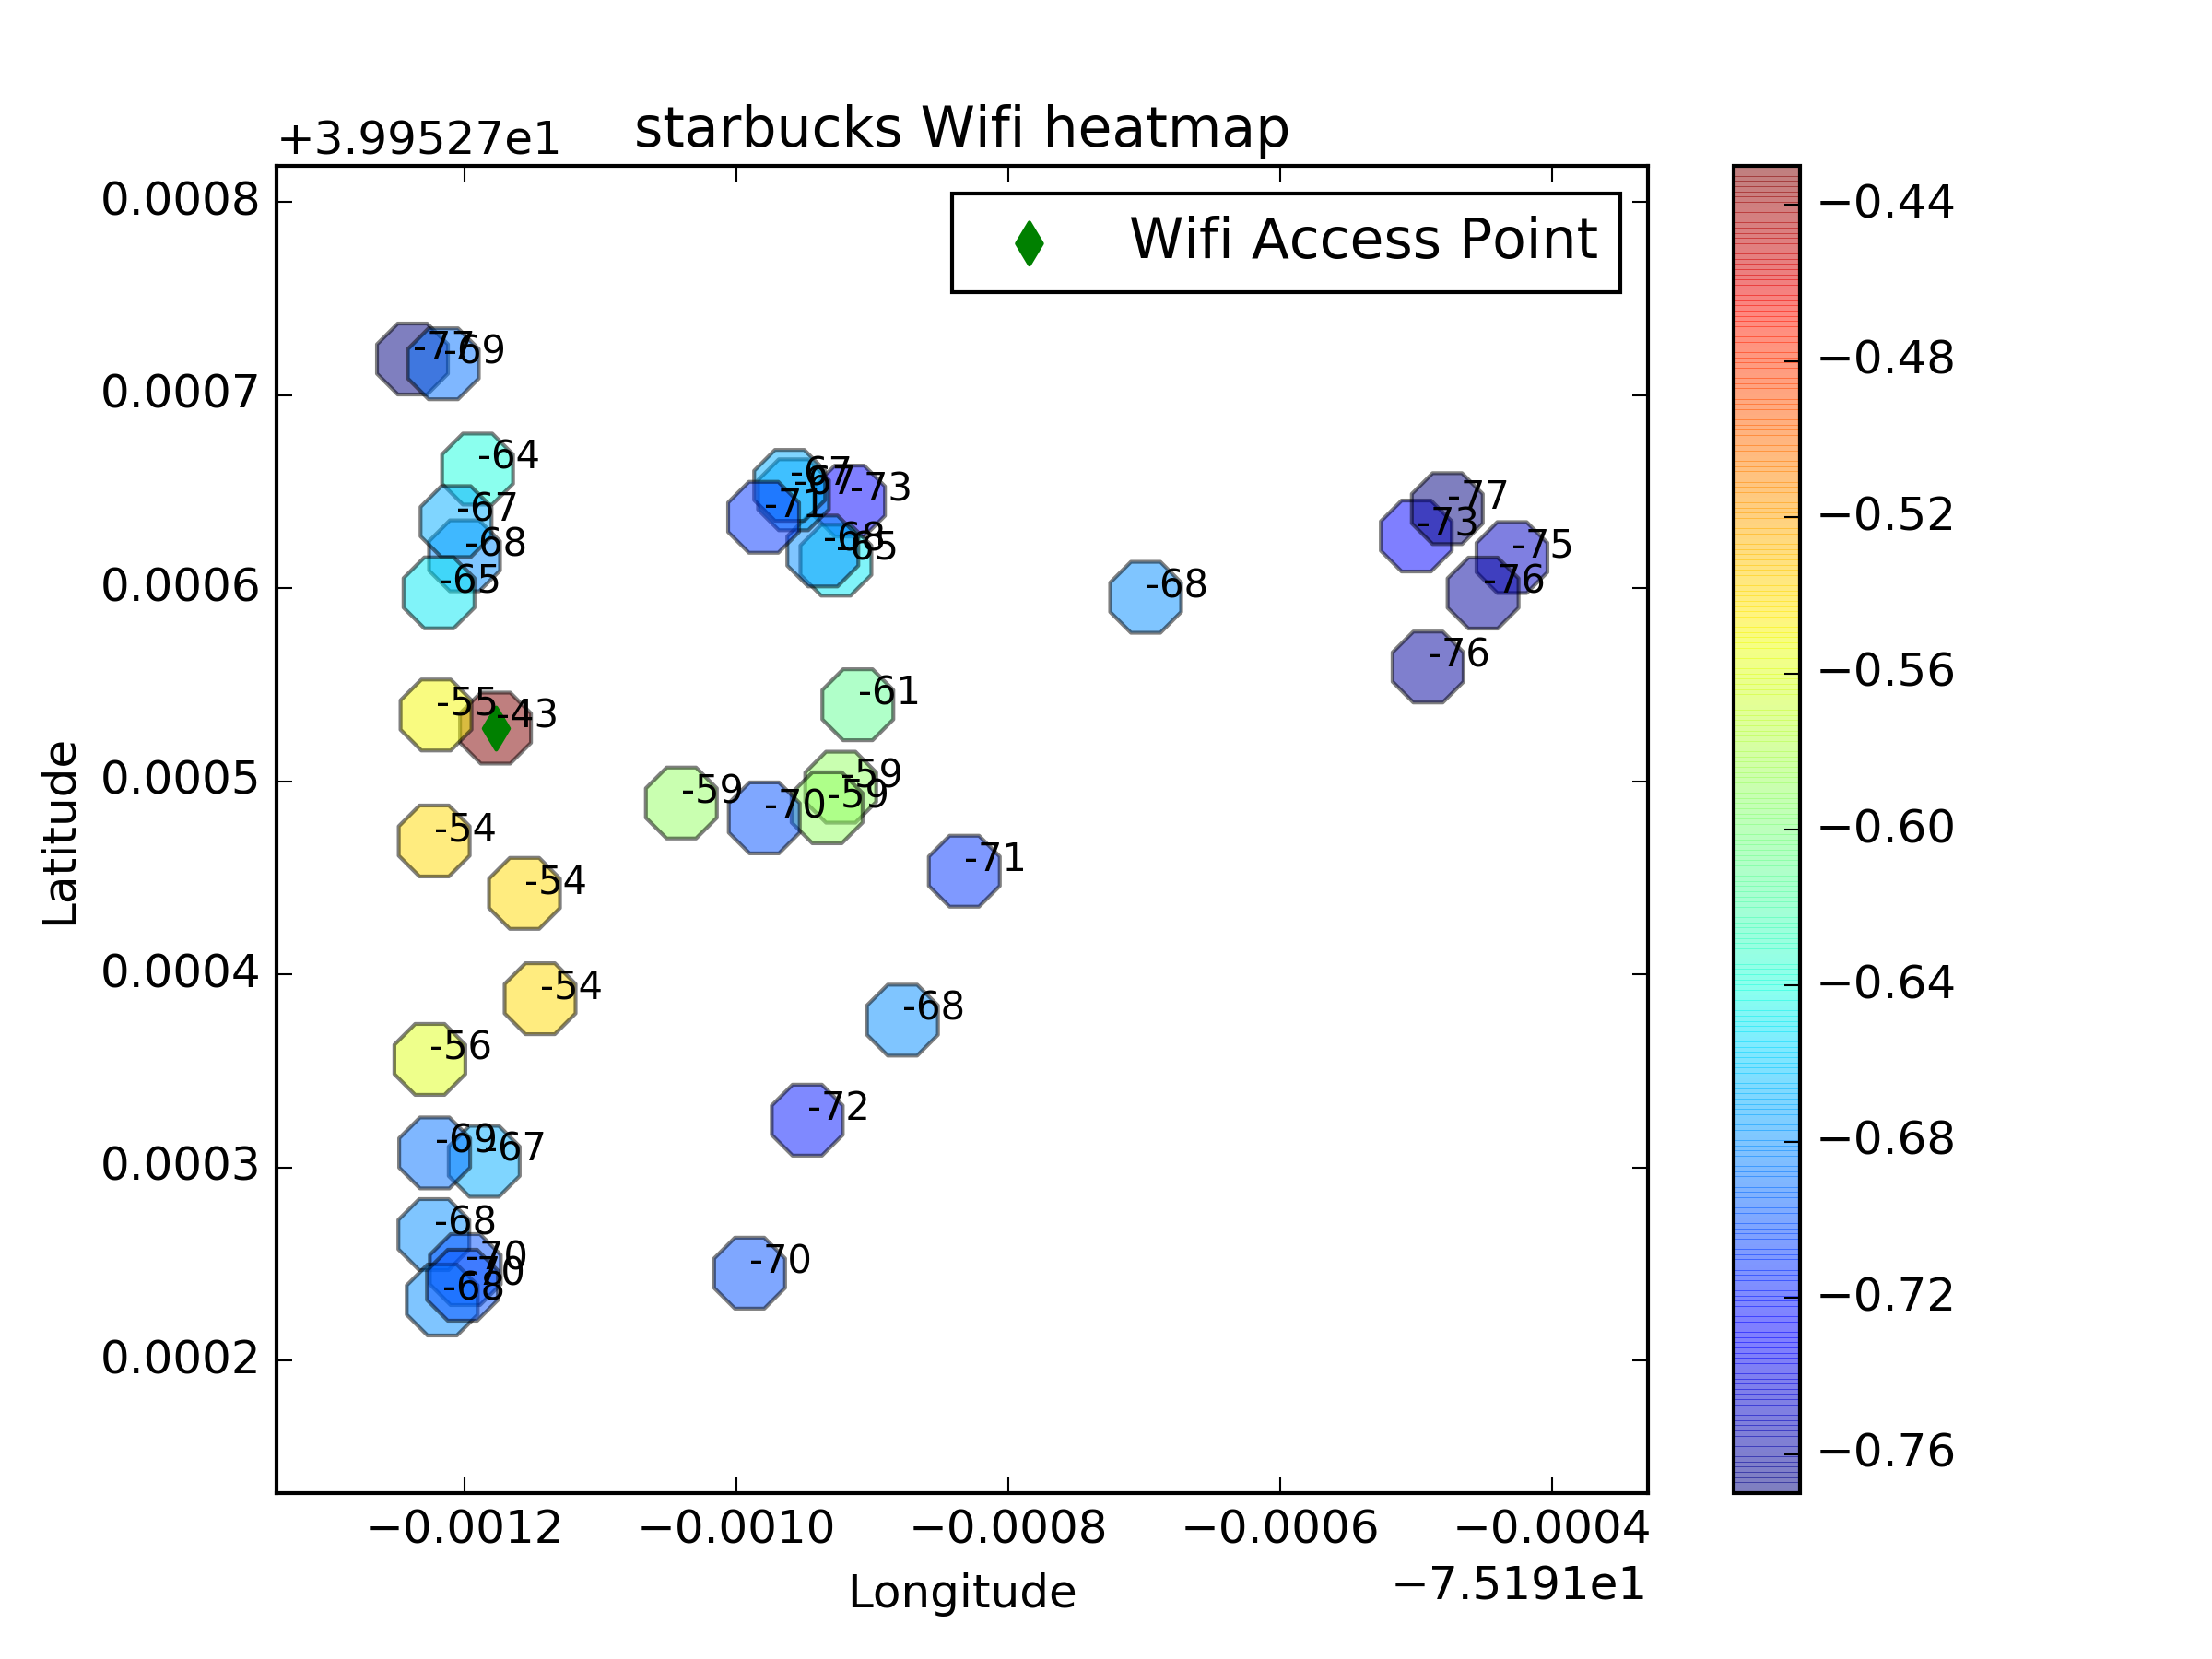
\includegraphics[width=1\linewidth, height=6cm]{starbucks.png}
		\caption{Starbucks Heat map}
	\end{subfigure}
	\caption{Library and Starbucks Heat map}
	\label{fig:plot7&8}
\end{figure}
\begin{figure}[!h]
	\begin{subfigure}{0.5\textwidth}
		\centering
		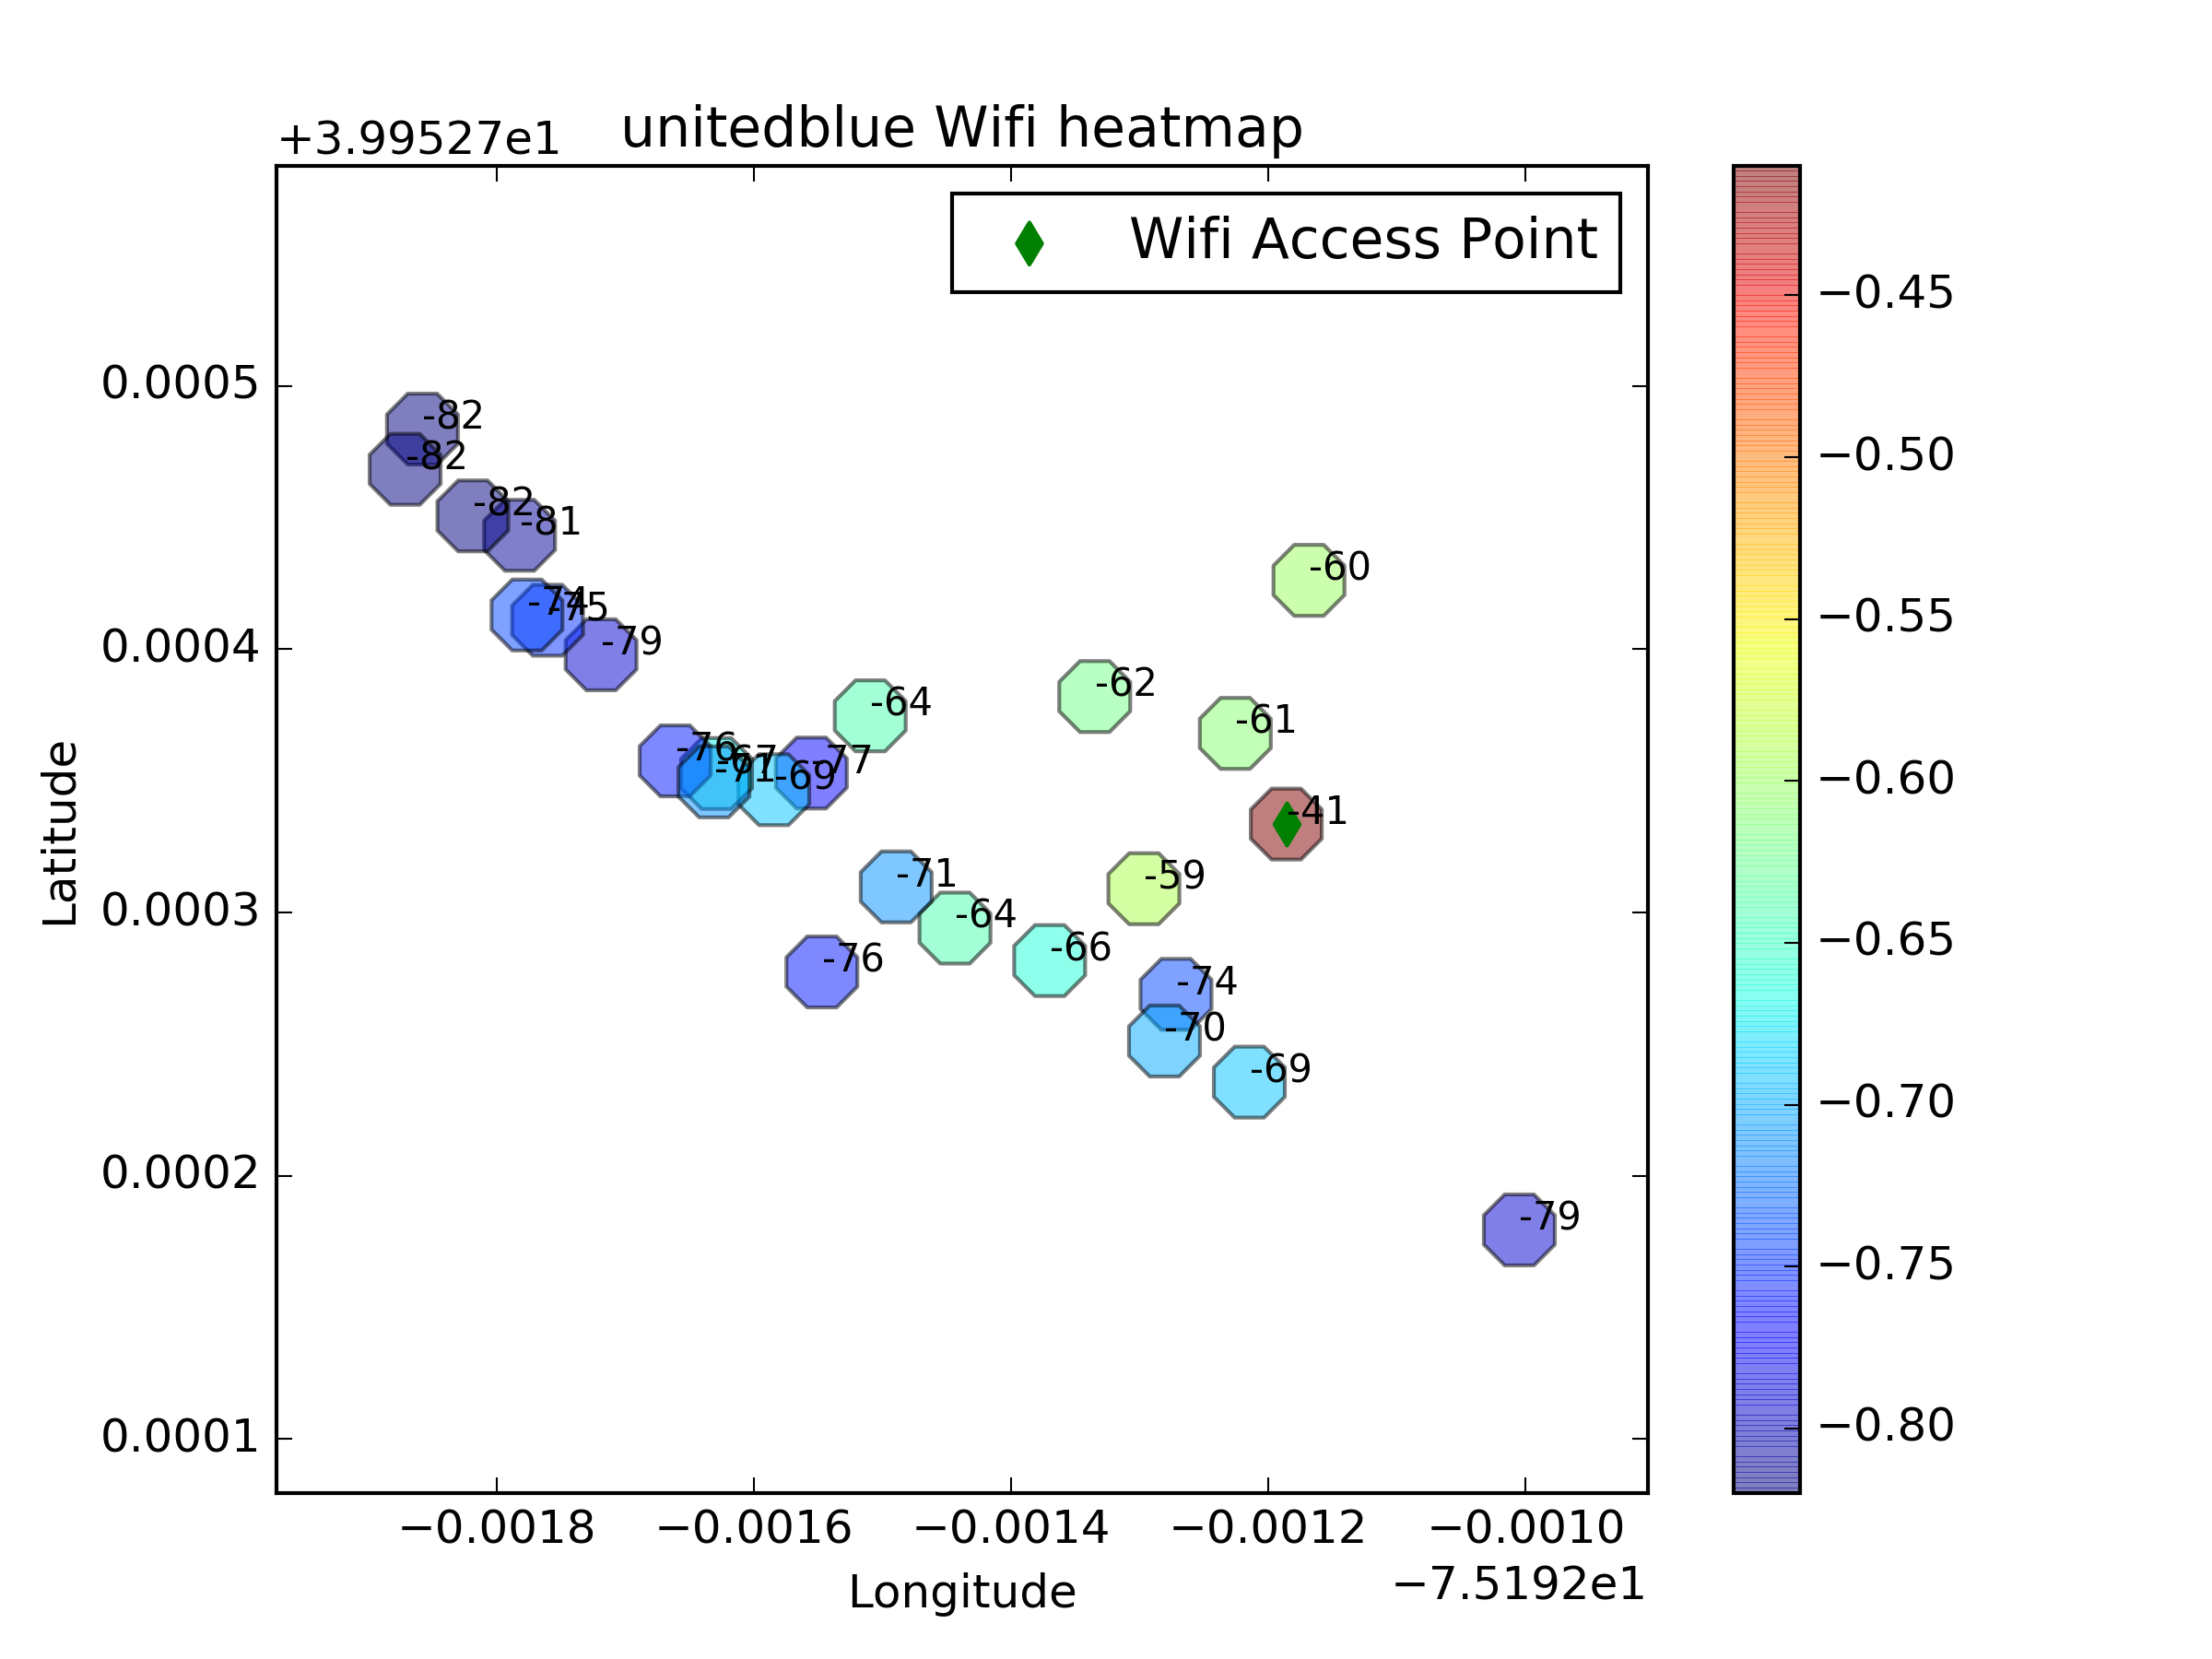
\includegraphics[width=1\linewidth, height=6cm]{unitedblue.png} 
		\caption{United by Blue Heat map}
	\end{subfigure}
	\begin{subfigure}{0.5\textwidth}
	    \centering
		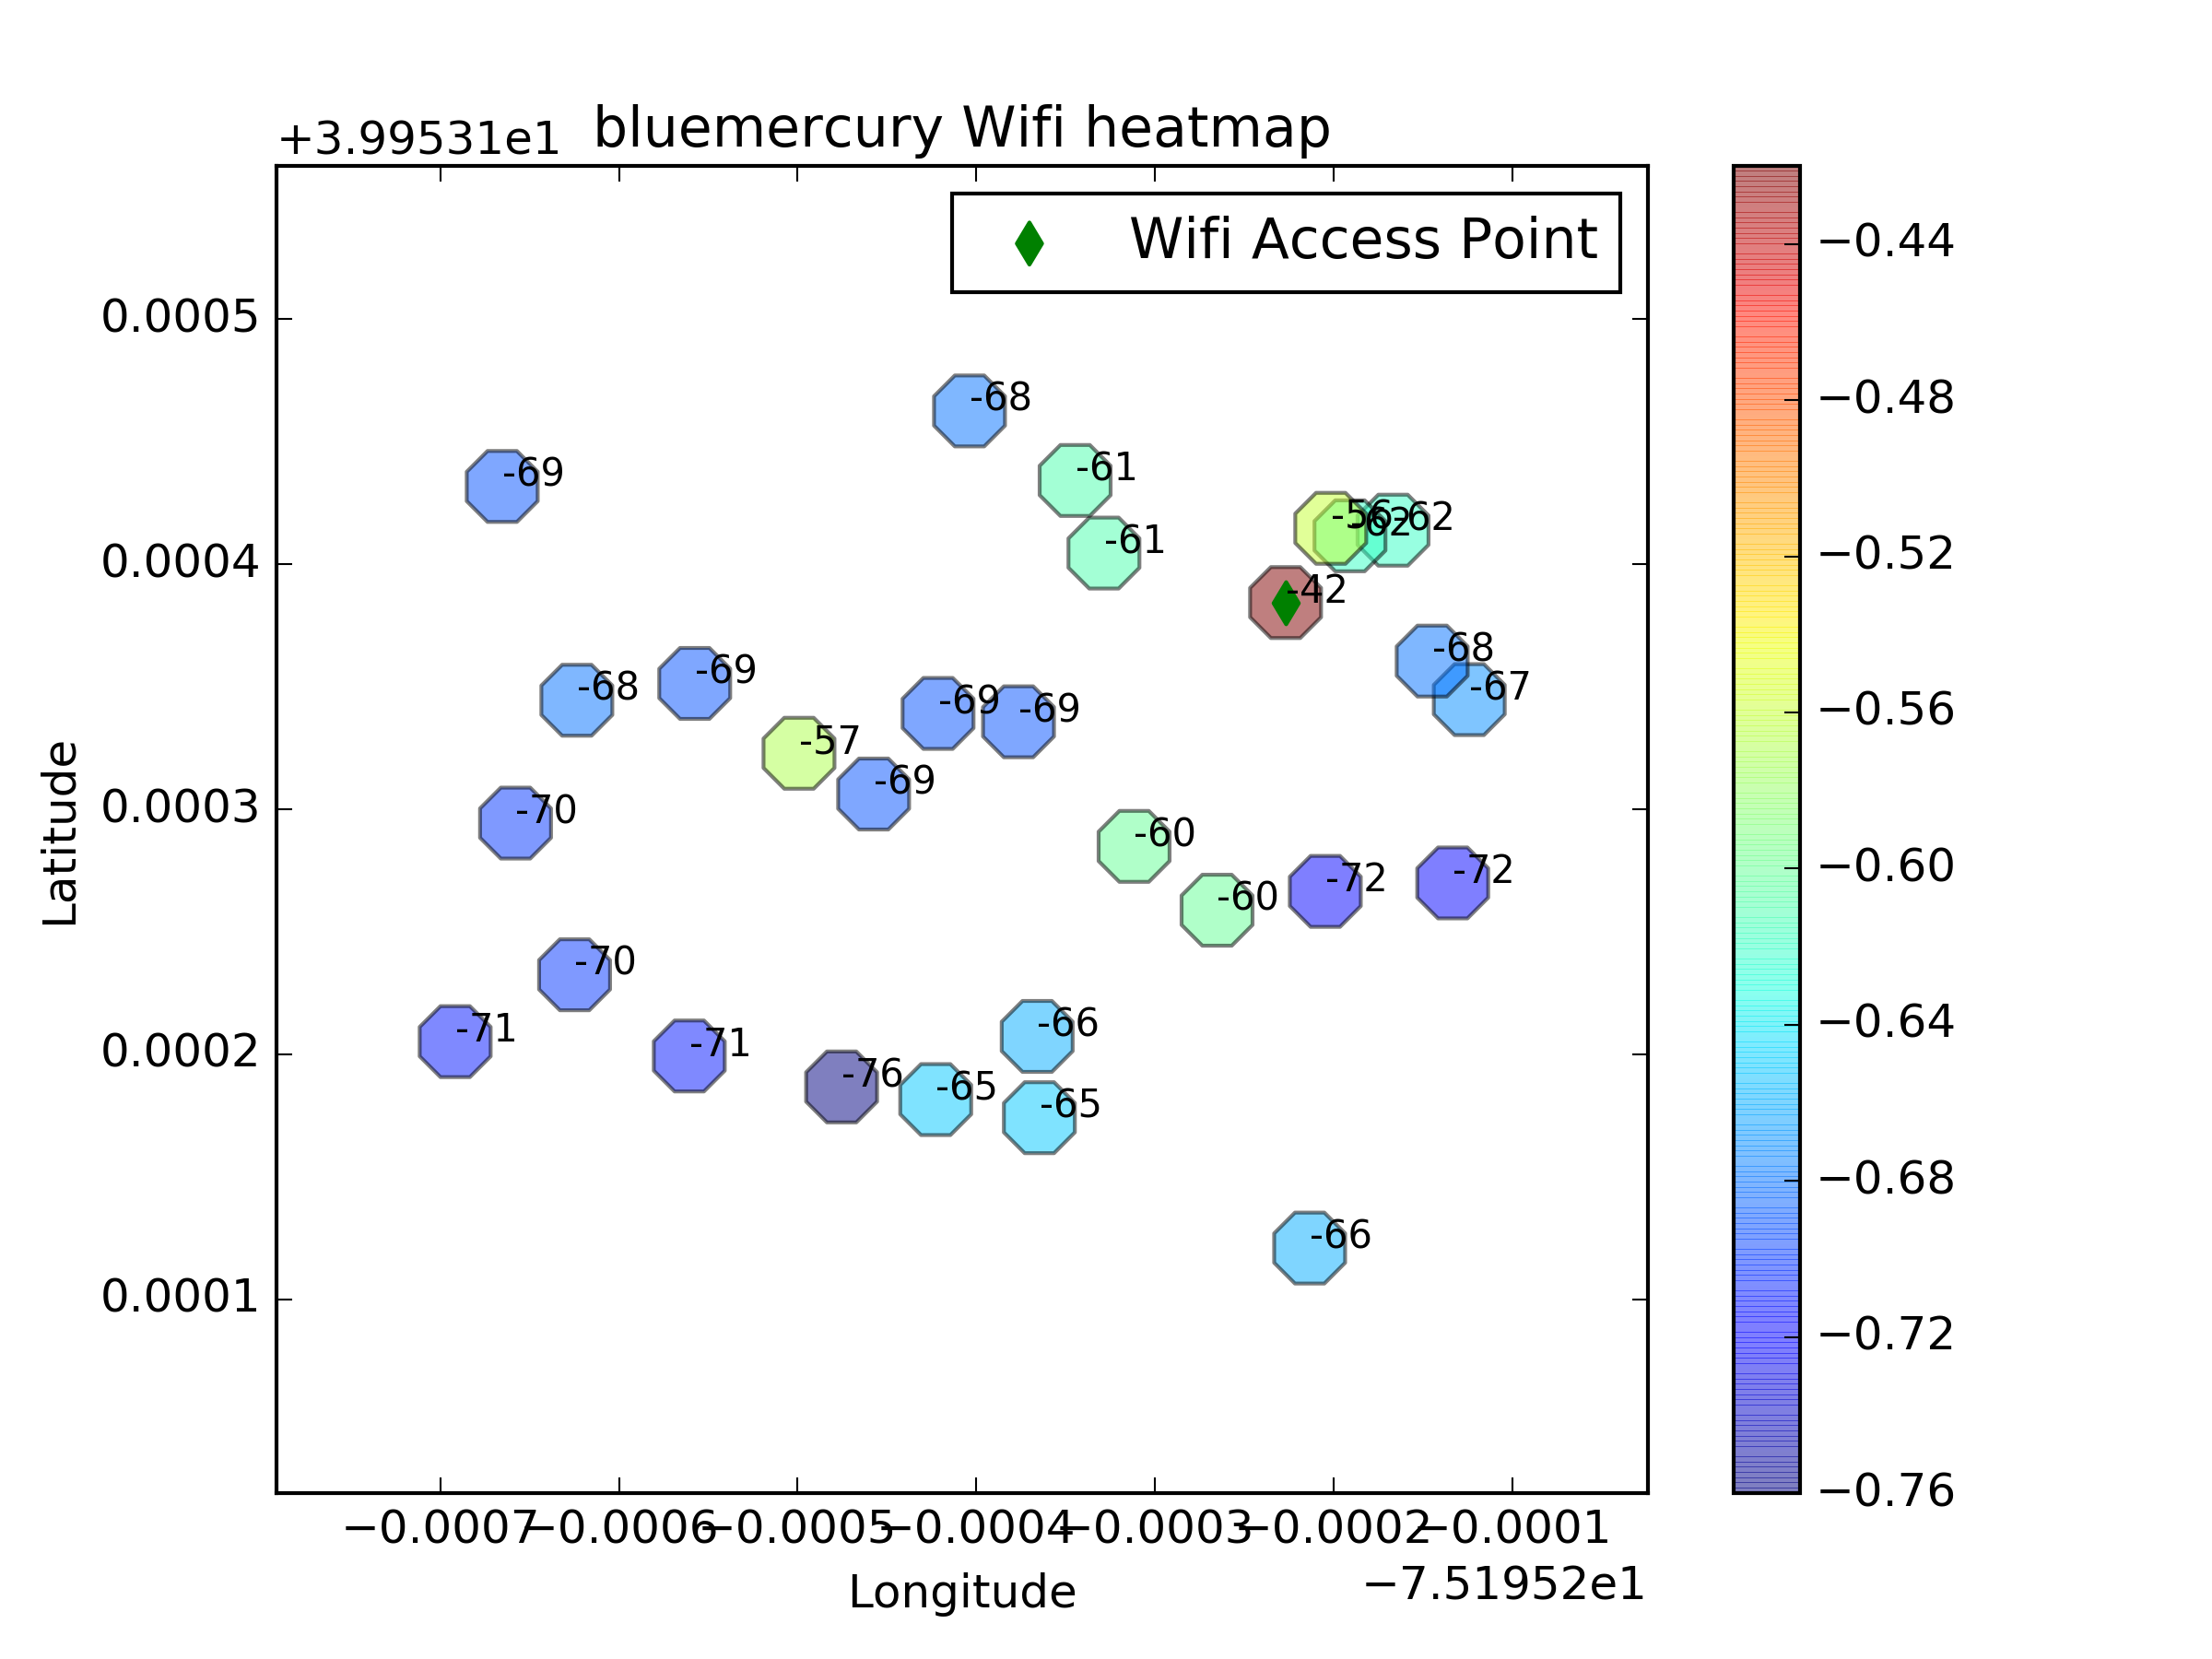
\includegraphics[width=1\linewidth, height=6cm]{bluemercury.png}
		\caption{Bluemercury Heat map}
	\end{subfigure}
	\caption{United by Blue and Bluemercury Heat map}
	\label{fig:plot9&10}
\end{figure}
\begin{figure}[!h]
	\centering
	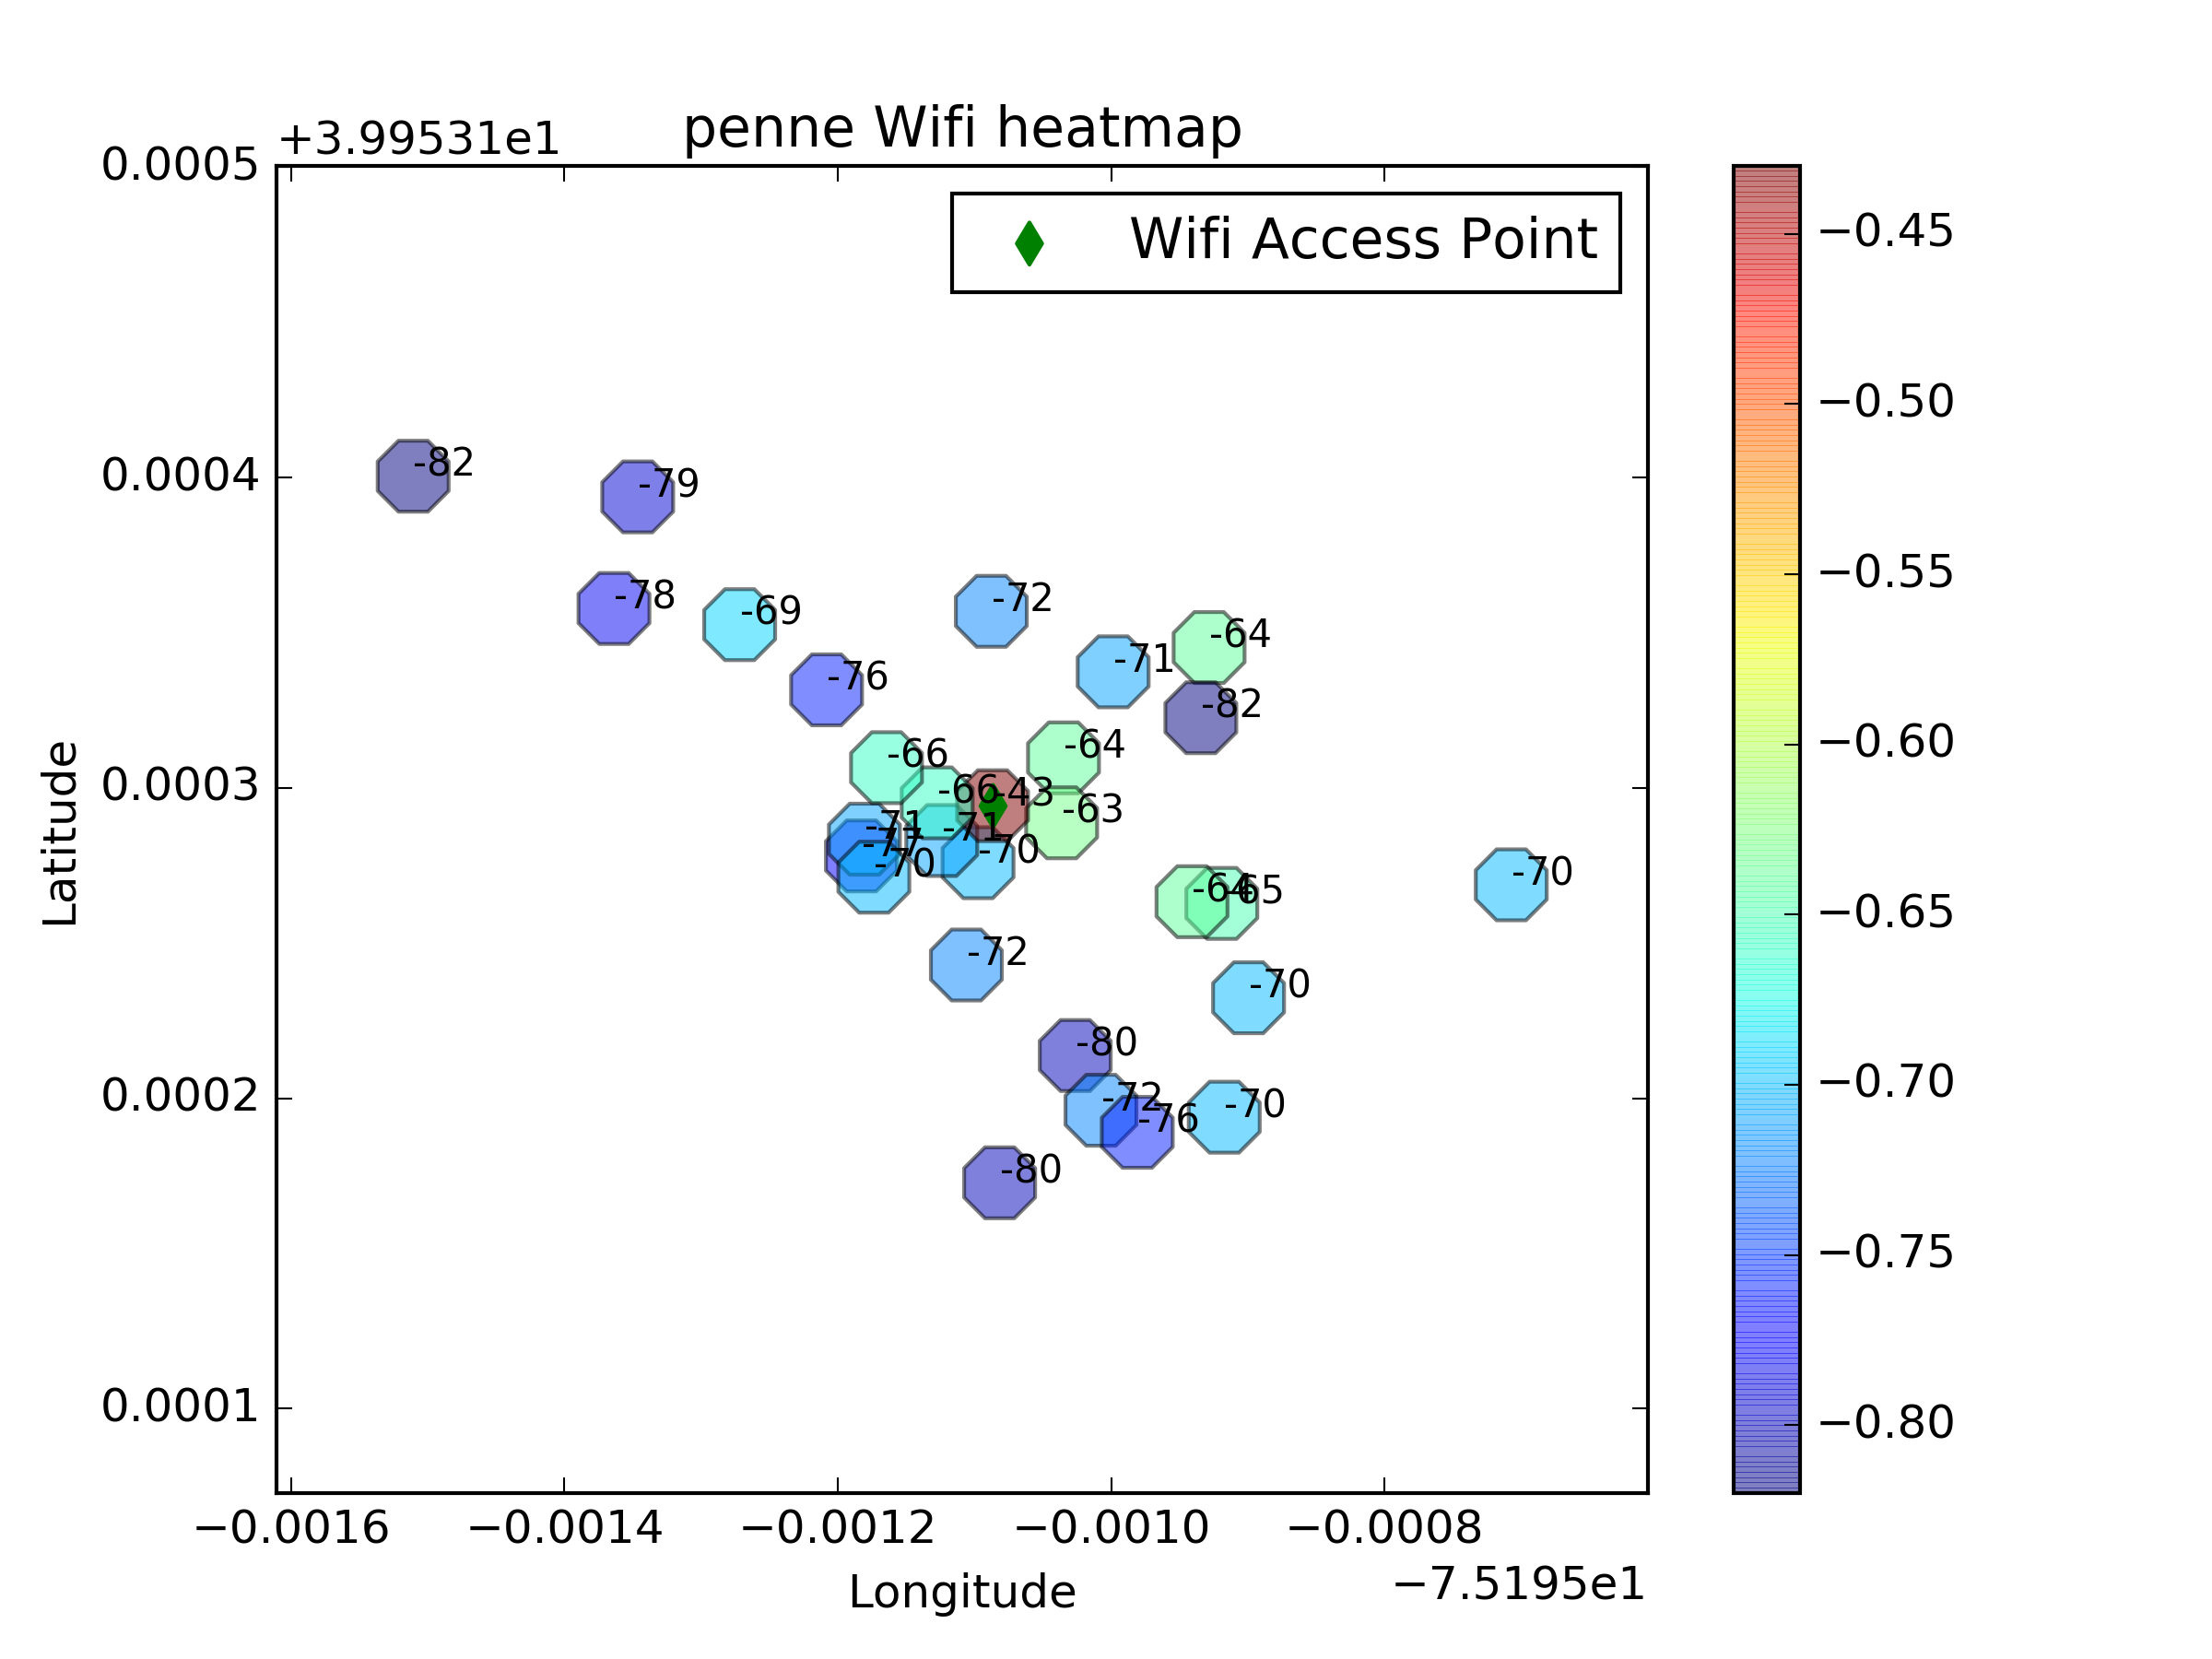
\includegraphics[width=1\linewidth]{penne.png}
	\caption{Penne-bar Heat map}
\label{fig:plot11}
\end{figure}
\clearpage

\section{Appendix: Python Source Code for data processing}
In the Appendix, as for reference, we attached the python code that analyzed and visualized the data for this whole project.
\lstinputlisting[language=Python,  breaklines=true,caption=WAP1\_Library]{phase2.py}
\end{document}